\documentclass[mti,article,submit,moreauthors]{Definitions/mdpi}

%=================================================================
% MDPI internal commands - do not modify
\firstpage{1}
\makeatletter
\setcounter{page}{\@firstpage}
\makeatother
\pubvolume{1}
\issuenum{1}
\articlenumber{0}
\pubyear{2026}
\copyrightyear{2026}
\datereceived{ }
\daterevised{ }
\dateaccepted{ }
\datepublished{ }
\externalbibliography{yes}



\renewcommand{\topfraction}{0.92}
\renewcommand{\bottomfraction}{0.85}
\renewcommand{\textfraction}{0.06}
\renewcommand{\floatpagefraction}{0.80}
\setcounter{topnumber}{3}
\setcounter{bottomnumber}{2}
\setcounter{totalnumber}{4}

%=================================================================
\Title{Temporal Validity and Sampling Bias in Pedestrian Crossing Prediction: A Multi-Dataset Audit and Controlled Evaluation}

% ORCID was not supplied for the first author and is therefore omitted.
\newcommand{\orcidauthorB}{0009-0003-4093-6946}
\newcommand{\orcidauthorC}{0000-0003-3150-0510}

\Author{Md. Arif Shekh $^{1}$, Nusrath Tabassum $^{1,2}$*\orcidB{}, Md Abdus Samad Kamal $^{2}$\orcidC{} and Kou Yamada $^{2}$}

\AuthorNames{Md. Arif Shekh, Nusrath Tabassum, Md Abdus Samad Kamal and Kou Yamada}

\address{%
$^{1}$ \quad Department of Computer Science and Engineering, International University of Business Agriculture and Technology, Dhaka, Bangladesh\\
$^{2}$ \quad Graduate School of Science and Technology, Gunma University, Kiryu 376-8515, Japan}

\corres{Correspondence: nusrathtabassum13@gmail.com}

\begin{abstract}{
Pedestrian crossing prediction aims to identify whether a pedestrian will cross before the crossing action begins. The temporal construction of the observation window is critical because frames from the crossing action can provide information about the event being predicted. This study examines the temporal validity of pedestrian crossing prediction samples in the PIE, JAAD, and IDD-PeD datasets. A frame-level audit shows that the original observation windows contain at least one crossing frame in 67.9\%, 93.0\%, and 81.3\% of positive samples, respectively. To avoid this overlap, the observation windows are reconstructed using the annotated crossing event. Although this removes crossing frames from the input, crossing and non-crossing pedestrians are still sampled at different temporal positions within their tracks. On PIE, a phase-matched control is used to reduce this difference by selecting non-crossing observations at comparable temporal positions. Four temporal models are evaluated using pedestrian bounding boxes with and without ego-vehicle speed. Under event-based sampling, the vanilla RNN achieves a ROC-AUC of 0.948 and an F1-score of 0.849, while adding ego-vehicle speed increases PR-AUC by up to 0.219. With phase matching and Holm correction, none of the box-only versus box-plus-speed comparisons remain statistically supported, suggesting that the observed benefit of ego-vehicle speed depends on how the observation window is constructed.
}
\end{abstract}

\keyword{Pedestrian crossing prediction; Temporal validity; Benchmark evaluation; PIE dataset; Pedestrian safety}
%=================================================================
\begin{document}

\section{Introduction}
\label{sec:introduction}

Road traffic crashes remain a major cause of death worldwide. The World Health Organization
reports approximately 1.16 million road traffic deaths each year, and road traffic injuries
remain the leading cause of death among people aged 5--29~\citep{who2026factsheet,who2026roaddeaths}. Pedestrians are among the most vulnerable road users. In 2021, they accounted for 23\% of global road traffic deaths, corresponding to an estimated 274,000 fatalities~\citep{who2023roadsafety}. In the United States, pedestrian fatalities also remain well above the levels observed a decade ago. These figures underline the need for intelligent vehicle systems that can respond to pedestrian behaviour before a hazardous interaction develops. Figure~\ref{fig:stats} summarises the global and U.S. pedestrian fatality statistics.

\begin{figure}[htbp]
\centering
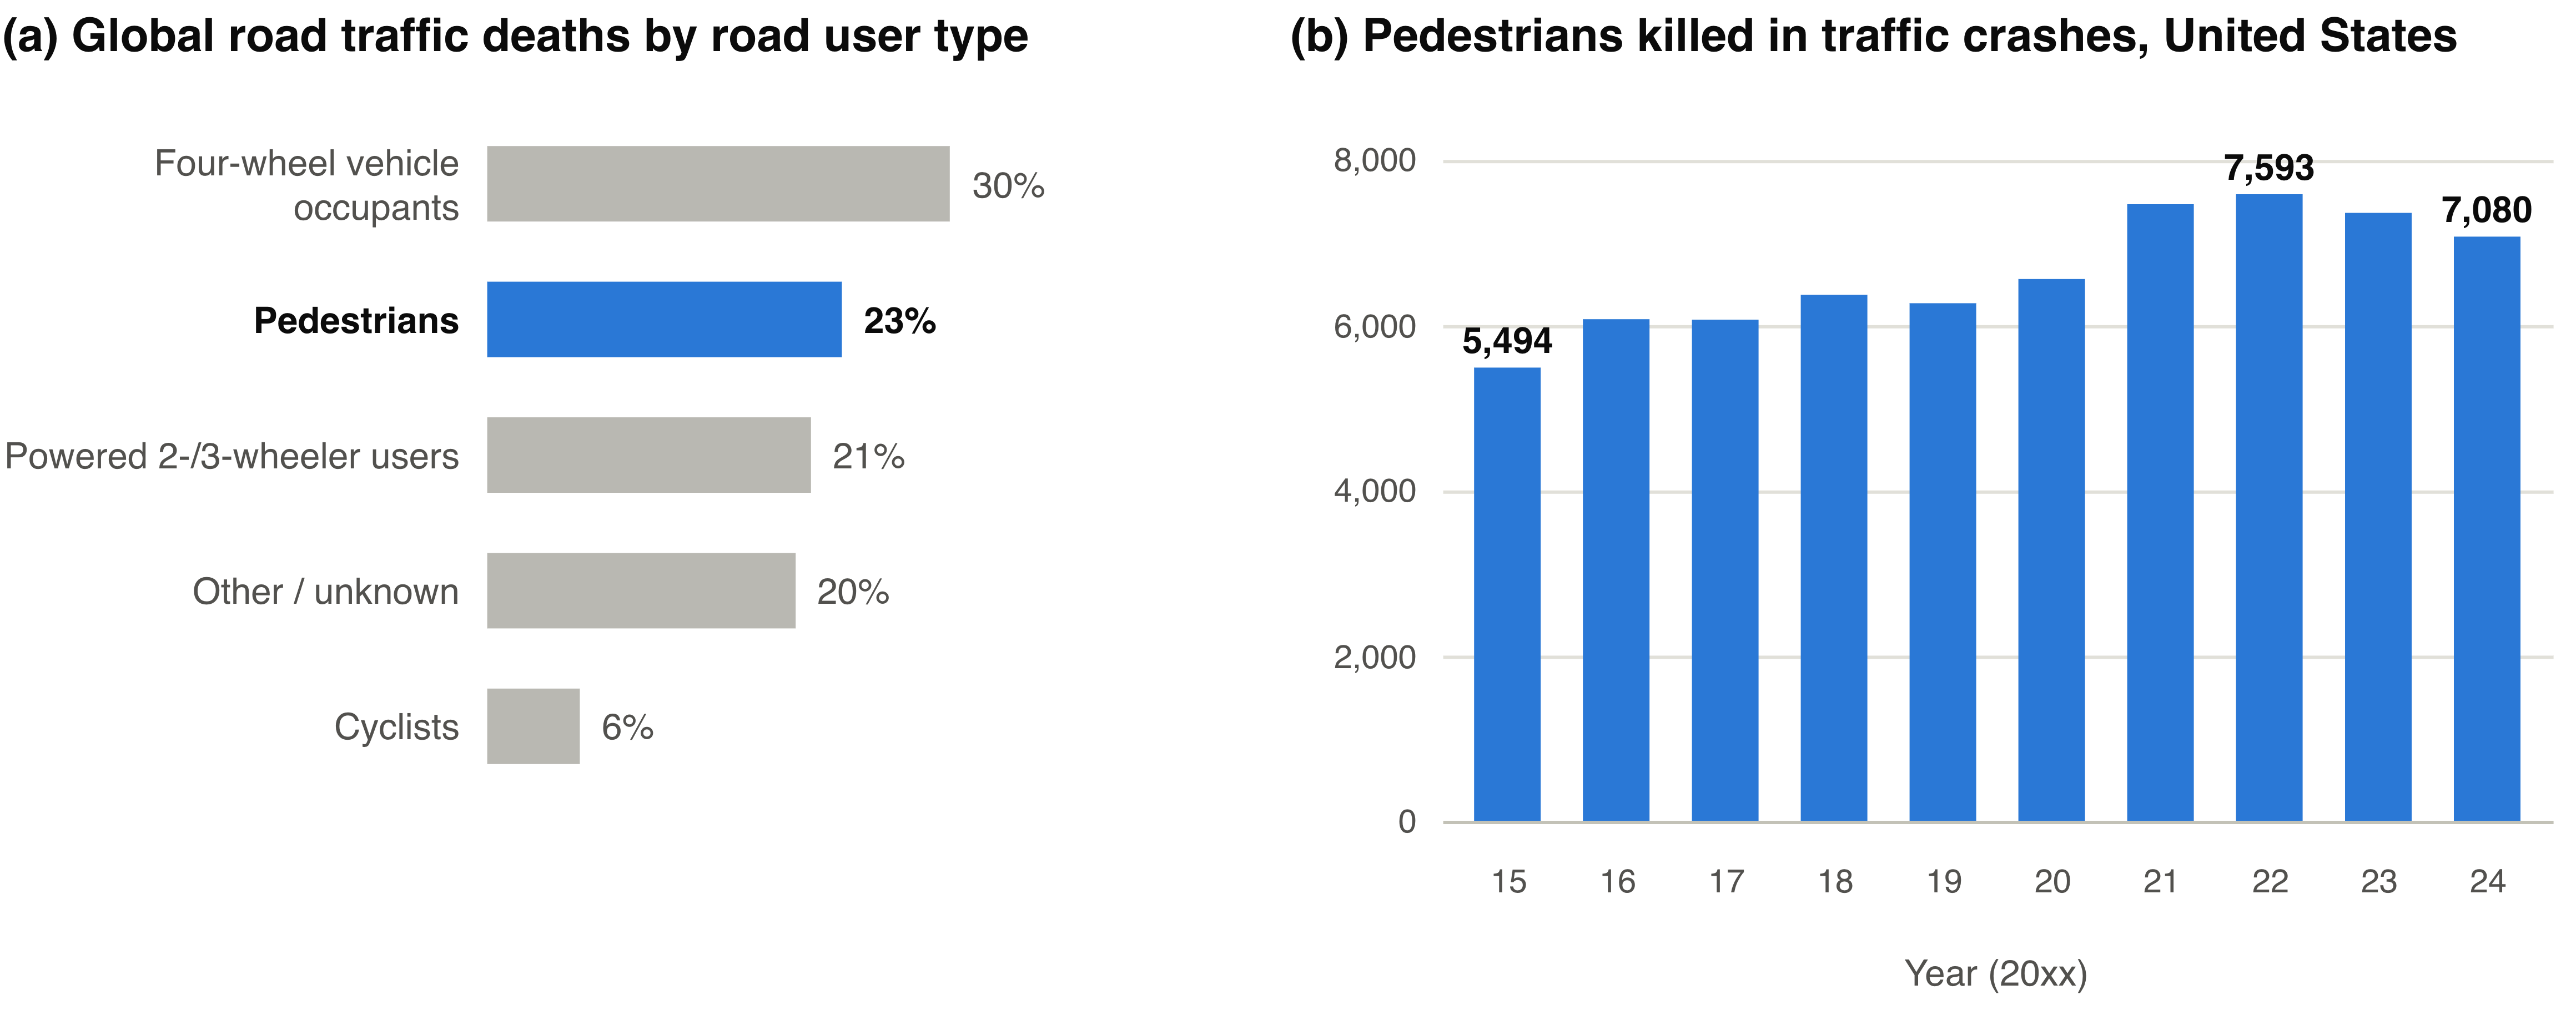
\includegraphics[width=\textwidth]{figures/fig1_pedestrian_statistics.png}
\caption{Pedestrian road fatalities. (\textbf{a}) Global road traffic deaths by road-user
type, 2021~\citep{who2023roadsafety}. (\textbf{b}) Pedestrians killed in United States
traffic crashes, 2015--2024~\citep{nhtsa2026pedestrian}.\label{fig:stats}}
\end{figure}

%Pedestrian detection alone is not enough for an intelligent vehicle system. The vehicle must also estimate whether a pedestrian is likely to enter its path before the crossing action begins.
\textcolor{red}{The prediction task depends on when the observation is made. An observation taken after a pedestrian has started crossing is fundamentally different from one taken before the crossing begins. Pedestrian detection alone is not enough for an intelligent vehicle system. It does not indicate whether a pedestrian is about to cross the road. For a driving system, this distinction is important because a crossing decision needs to be made before the pedestrian enters the vehicle's path. Pedestrian crossing prediction therefore uses observations of pedestrian movement to estimate a future crossing event. For such prediction, the timing of the observations is important. If the observation window already includes frames from the crossing action, the model receives information about an event that it is expected to predict. A valid prediction window should therefore represent the pedestrian's state before the crossing begins.} The literature often describes this problem as crossing-intention prediction,
although intention estimation and future action prediction are distinct
concepts~\citep{rasouli2024diving}.
The Pedestrian Intention Estimation (PIE) dataset~\citep{rasouli2019pie} is widely used
for pedestrian crossing prediction because it provides pedestrian tracks, behavioural annotations, bounding boxes, vehicle information, and annotated crossing events. The
established PIE action-prediction benchmark uses a fixed observation period and a future
time-to-event interval so that prediction is evaluated before the crossing event
~\citep{kotseruba2021benchmark}. The protocol defines when a prediction should be made,
but the nominal prediction horizon alone does not show whether every generated observation
window actually contains only pre-crossing information.

This distinction motivates the first problem examined in this study. If an extraction
procedure positions an observation relative to the end of a pedestrian track rather than the
crossing onset, part of the crossing action may already appear inside the input sequence. An
event marker can also differ from the first frame at which crossing is observed. Comparing
each observed frame with the annotated crossing state therefore provides a direct test of
whether the generated samples remain pre-event. 
%Removing crossing frames from positive observations does not necessarily remove every temporal shortcut. 
\textcolor{red}{Removing crossing frames from positive observations does not necessarily remove all information introduced by the sampling procedure.} Crossing pedestrians have a behavioural event that provides a natural
reference point, whereas non-crossing pedestrians have no equivalent future crossing event.
If the negative class is anchored close to the end of the pedestrian track, the two classes may
be observed at systematically different stages of the pedestrian--vehicle interaction. This
temporal position is not supplied explicitly to the models, but it can be reflected through
pedestrian scale, relative motion, and ego-vehicle speed. The sampling rule can therefore
affect the information available for prediction even when every positive observation occurs
before crossing onset.

The issue is particularly relevant to ego-vehicle speed. Previous PIE-based studies report that bounding-box geometry and ego-vehicle motion can provide strong predictive information
~\citep{lorenzo2021intformer,azarmi2024featureimportance,chen2024pedcmt}. If the two classes are observed at different temporal phases, part of the apparent contribution of vehicle speed may come from this sampling structure rather than from a stable relationship that persists after temporal control. The contribution of ego-vehicle speed should therefore be examined under both the event-anchored and phase-controlled protocols. \textcolor{red}{The same temporal issue is relevant when comparing model architectures.} Pedestrian crossing prediction has been studied with recurrent networks, attention mechanisms, graph models, and Transformers. Direct comparison across papers is difficult because the models often use different inputs, preprocessing, tuning budgets, and training procedures. A controlled comparison should keep these conditions fixed while changing the neural temporal model. It is then possible to examine whether the apparent differences between model families remain when the temporal sampling procedure is changed.

These considerations lead to three research questions. First, are the generated observation windows temporally valid when checked directly against frame-level crossing onset, and does the same conclusion hold across PIE, JAAD, and IDD-PeD? Second, after direct crossing-frame contamination is removed, does class-dependent temporal sampling remain, and how does controlling this sampling phase affect model performance and the contribution of ego-vehicle speed? Third, \textcolor{red}{do the relative performance differences among BiLSTM, GRU, vanilla RNN, and Transformer models remain consistent under different temporal sampling protocols?}

\textcolor{red}{To address these questions, PIE is used as the primary controlled benchmark, while JAAD and IDD-PeD provide external temporal checks, with IDD-PeD also supporting cross-dataset evaluation.} The generated windows are first audited against frame-level crossing annotations. PIE is then rebuilt using the annotated crossing event, after which the remaining class-dependent temporal phase is measured and reduced through a phase-matched negative control. The same four neural model families are evaluated with pedestrian bounding boxes and ego-vehicle speed, and the speed channel is ablated under both PIE sampling protocols.

This study makes the following contributions:

\begin{itemize}
\item The common observation windows of PIE, JAAD, and IDD-PeD are audited frame by frame against each dataset's own crossing annotation, instead of trusting a nominal prediction horizon or the presence of an event marker. \textcolor{red}{The audit shows that windows anchored on the end of a pedestrian track already contain the action to be predicted, and this issue is not specific to one dataset. This provides a way to check whether a benchmark is pre-event before model training.}

\item \textcolor{red}{Anchoring the observation window to the annotated crossing onset removes direct overlap with the crossing action on PIE, but the sampling procedure can still place crossing and non-crossing observations at different temporal positions within their tracks. This residual difference is measured by the distance between the observation window and the end of the pedestrian track. A phase-matched control then shifts the non-crossing windows earlier using a distribution estimated from the training positives alone. This reduces the temporal difference between the two classes and allows the effect of the sampling procedure to be evaluated more directly.
}

\item \textcolor{red}{The two input modalities, pedestrian bounding-box geometry and ego-vehicle motion, are evaluated separately under both sampling rules, with the same data partitions, configurations, and random seeds used for each comparison. The statistical comparison supports an effect of ego-vehicle speed before phase matching, but not after phase matching. This indicates that the measured contribution of ego-vehicle speed is sensitive to the temporal sampling of the two classes and should therefore be interpreted together with the sampling protocol.}

\item \textcolor{red}{BiLSTM, GRU, vanilla RNN, and Transformer encoders are compared using the same data, preprocessing, training–validation separation, and test-evaluation procedures, with five random seeds, pedestrian-clustered bootstrap resampling over 10,000 replicates, and Holm–Bonferroni correction within a predefined family of comparisons. Differences between the model architectures that are statistically supported under the original sampling protocol are no longer supported after temporal control. This indicates that the observed differences between model architectures are sensitive to the temporal sampling protocol used to construct the benchmark.}
\end{itemize}



The remainder of this paper is organized as follows. %Section~\ref{sec:related_work} reviews benchmark construction, input information, temporal modeling, and evaluation reliability for pedestrian crossing prediction. Section~\ref{sec:methods} describes the datasets, the two temporal extraction procedures, the phase-matched negative control, the input representation, and the four neural model families. Section~\ref{sec:experimental-settings} gives the computing environment, the training and model-selection configuration, and the statistical procedure. Section~\ref{sec:results} reports the frame-level temporal audit across the three datasets, the four-family comparison, and the ego-speed ablation under both sampling protocols. Section~\ref{sec:discussion} interprets these results, Section~\ref{sec:limitations} states the limitations, and Section~\ref{sec:conclusions} concludes.
\textcolor{red}{Section~\ref{sec:related_work} reviews related work. Section~\ref{sec:methods} describes the datasets, the two temporal extraction procedures, the phase-matched control, the input representation, and the four temporal model architectures. Section~\ref{sec:experimental-settings} presents the computing environment, training and model-selection configuration, and statistical procedure. Section~\ref{sec:results} reports the frame-level temporal audit across the three datasets, the comparison of the four temporal architectures, and the ego-vehicle speed ablation under both sampling protocols. Section~\ref{sec:discussion} interprets the results, Section~\ref{sec:limitations} discusses the limitations, and Section~\ref{sec:conclusions} concludes the paper.
}

\section{Related Work}
\label{sec:related_work}

Pedestrian behaviour prediction covers several related tasks, including intention estimation, future crossing-action prediction, and trajectory prediction. The present study concerns future crossing action. The related literature is reviewed from four perspectives that directly affect how this task is evaluated: benchmark construction, input information, temporal modeling, and evaluation reliability.

\subsection{Benchmark Semantics and Temporal Evaluation}

JAAD provided one of the early large-scale resources for studying pedestrian behaviour from a vehicle perspective, with pedestrian tracks and behavioural and contextual annotations~\citep{rasouli2017jaad}. PIE later extended this setting with a larger continuous driving dataset, pedestrian bounding boxes, behavioural annotations, human-reference intention data, and synchronised ego-vehicle information~\citep{rasouli2019pie}. The two datasets have subsequently supported studies described using terms such as pedestrian intention, crossing behaviour, and action prediction. Rasouli and Kotseruba~\citep{rasouli2024diving} clarified that these terms should not be used interchangeably: intention refers to a latent state, whereas action prediction concerns a future observable behaviour. A major step toward consistent action-prediction evaluation was introduced by Kotseruba et al.~\citep{kotseruba2021benchmark}. Their benchmark defined the prediction event as the start of crossing for a positive pedestrian and the last observable frame for a pedestrian who did not cross. Observations were taken before this event, with a fixed observation length and a time-to-event interval. The same work also showed that earlier studies differed substantially in whether observations were restricted to the pre-crossing period or sampled from the full pedestrian trajectory. It explicitly noted that prediction was no longer meaningful once the action was already in progress.

This benchmark is important prior work for the present study because the principle of pre-event prediction is already established. The remaining question is whether the samples generated from a particular implementation or annotation set actually satisfy that principle. The benchmark paper did not report a frame-by-frame audit of generated observations against the crossing state. It also defined the temporal event differently for crossing and non-crossing pedestrians, but did not quantify whether these class-dependent anchors placed the classes at systematically different phases of their tracks.


\subsection{Input Information and Restricted Representations}

Pedestrian crossing models have used increasingly diverse sources of information. Multimodal approaches have combined pedestrian appearance, bounding-box motion, body pose, scene context, semantic information, and ego-vehicle dynamics. PCPA combined visual and non-visual pedestrian and vehicle information~\citep{kotseruba2021benchmark}; BiPed jointly predicted pedestrian trajectory and crossing action from multimodal contextual representations~\citep{rasouli2021biped}; and PedFormer used cross-modal attention together with pedestrian--traffic interactions for trajectory and action prediction~\citep{rasouli2023pedformer}. Other methods, including PIT, PIP-Net, GTransPDM, and MFT, extended this direction through Transformer, graph-based, recurrent, and contextual fusion mechanisms~\citep{zhou2023pit,azarmi2025pipnet,xie2025gtranspdm,li2025mft}.

At the same time, strong performance was also reported with much smaller input sets. PedCMT used only pedestrian bounding boxes and ego-vehicle speed and reported performance comparable with approaches using richer inputs~\citep{chen2024pedcmt}. Achaji et al.~\citep{achaji2022attention} showed that a Transformer operating only on bounding-box sequences could achieve strong PIE action-prediction performance. EfficientPIE reduced the temporal input further and reported similar performance using a single pedestrian image rather than a sequence of observed images~\citep{qu2025efficientpie}. These studies showed that complex multimodal input was not always necessary for strong benchmark performance.

Ego-vehicle speed received particular attention within these restricted representations. IntFormer reported ego speed as its strongest individual input and found the combination of bounding-box coordinates and speed particularly effective~\citep{lorenzo2021intformer}. The context-aware feature-importance analysis of Azarmi et al.~\citep{azarmi2024featureimportance} similarly identified bounding boxes as the most important feature and ego speed as another major contributor across several model architectures. That study also reported potential prediction bias associated with the speed feature and motivated a representation based more directly on pedestrian--vehicle proximity change. These findings showed that bounding-box geometry and ego motion could carry substantial predictive information. They did not, however, determine how much of that information depended on the temporal rule used to construct positive and negative samples.


\subsection{Temporal Models and Controlled Comparison}

Recurrent networks were widely used in earlier pedestrian action-prediction systems because
they provide a direct way to represent motion over an observation sequence. Later work
introduced attention mechanisms, graph representations, and Transformer architectures to
capture longer-range temporal relations and interactions between different input modalities
~\citep{kotseruba2021benchmark,cadena2022pedgraph,lorenzo2021intformer,
zhou2023pit,rasouli2021biped,rasouli2023pedformer,xie2025gtranspdm}. These models
differ not only in their temporal encoders but also in their input modalities, parameter
counts, preprocessing, optimisation, and model-selection procedures.

For this reason, reported scores from different papers cannot be interpreted as a direct comparison of temporal architecture alone. \textcolor{red}{Melis et al.~\citep{melis2018sota} showed that careful and comparable hyperparameter optimisation could substantially affect the relative performance of competing sequence models.} Lucic et al.~\citep{lucic2018gans} similarly demonstrated the importance of comparable computational and tuning budgets when evaluating model families. Greff et al.~\citep{greff2017odyssey} found that several commonly proposed LSTM architectural changes had relatively limited impact after systematic optimisation, while Chung et al.~\citep{chung2014gru} compared gated recurrent architectures under controlled sequence-modeling conditions. \textcolor{red}{These studies highlight the importance of controlled experimental conditions when comparing temporal architectures. The same principle applies to benchmark construction: if the temporal sampling procedure changes, the relative performance of the architectures may also change.}

\subsection{Evaluation Reliability and Cross-Dataset Generalization}

Reliable comparison also depends on the evaluation procedure. Pedestrian crossing datasets are class-imbalanced, so accuracy alone can hide important differences in positive-class performance. Precision--recall analysis is particularly informative under imbalance~\citep{davis2006precision,saito2015precision}. Model-selection procedures also need to separate configuration decisions from final testing because repeated use of evaluation data during selection can produce optimistic performance estimates~\citep{cawley2010overfitting}.

Model performance can also vary across training runs. \textcolor{red}{Reimers and Gurevych~\citep{reimers2017reporting} showed that reported performance can vary across training runs, while Bouthillier et al.~\citep{bouthillier2021variance} identified data sampling, parameter initialisation, and hyperparameter optimisation as important sources of benchmark variance.} A further issue arises when several observation windows come from the same pedestrian. Such observations form clusters rather than independent samples, motivating uncertainty estimates that preserve this dependence~\citep{fieldwelsh2007}. These considerations are important when differences between models are small relative to the variability of the benchmark.

Within-dataset evaluation also does not establish robustness to a different traffic domain. Gesnouin et al.~\citep{gesnouin2022assessing} directly evaluated pedestrian crossing predictors across datasets and found substantial degradation compared with conventional within-dataset testing. More recently, IDD-PeD was introduced to represent pedestrian behaviour in less structured traffic, including challenging illumination, occlusion, unsignalised scenes, and vehicle--pedestrian interactions~\citep{bokkasam2025iddped}. Existing intention-prediction methods also showed substantial performance degradation on this dataset. These findings make external evaluation important when interpreting conclusions obtained from PIE alone.

\textcolor{red}{The reviewed studies establish the importance of pre-event prediction and controlled model evaluation, but they do not examine whether the frames contained in commonly used observation windows remain entirely before the annotated crossing onset. They also do not quantify the difference in temporal position between crossing and non-crossing observations or examine how this difference affects comparisons of input modalities and temporal architectures. This study first audits the observation windows generated for PIE, JAAD, and IDD-PeD against their frame-level crossing annotations to identify direct overlap with the crossing action. Based on this audit, the observation windows are re-extracted by anchoring them to the annotated crossing onset, thereby removing direct crossing-frame contamination. Because event anchoring does not eliminate the difference in temporal position between crossing and non-crossing observations, a phase-matched control is then constructed for PIE to reduce this remaining difference. The controlled sampling protocols are used to evaluate pedestrian bounding-box geometry and ego-vehicle speed separately and to compare BiLSTM, GRU, vanilla RNN, and Transformer models under the same experimental conditions. Cross-dataset testing on IDD-PeD further examines whether the findings obtained from PIE extend to a different traffic environment.
}

\section{Materials and Methods}\label{sec:methods}
This section describes the dataset, temporal data extraction, input representation, prediction models, and training and evaluation procedures used in the study. Figure~\ref{fig:method} summarises the complete pipeline from an annotated pedestrian track
to a crossing prediction.
\begin{figure}[H]
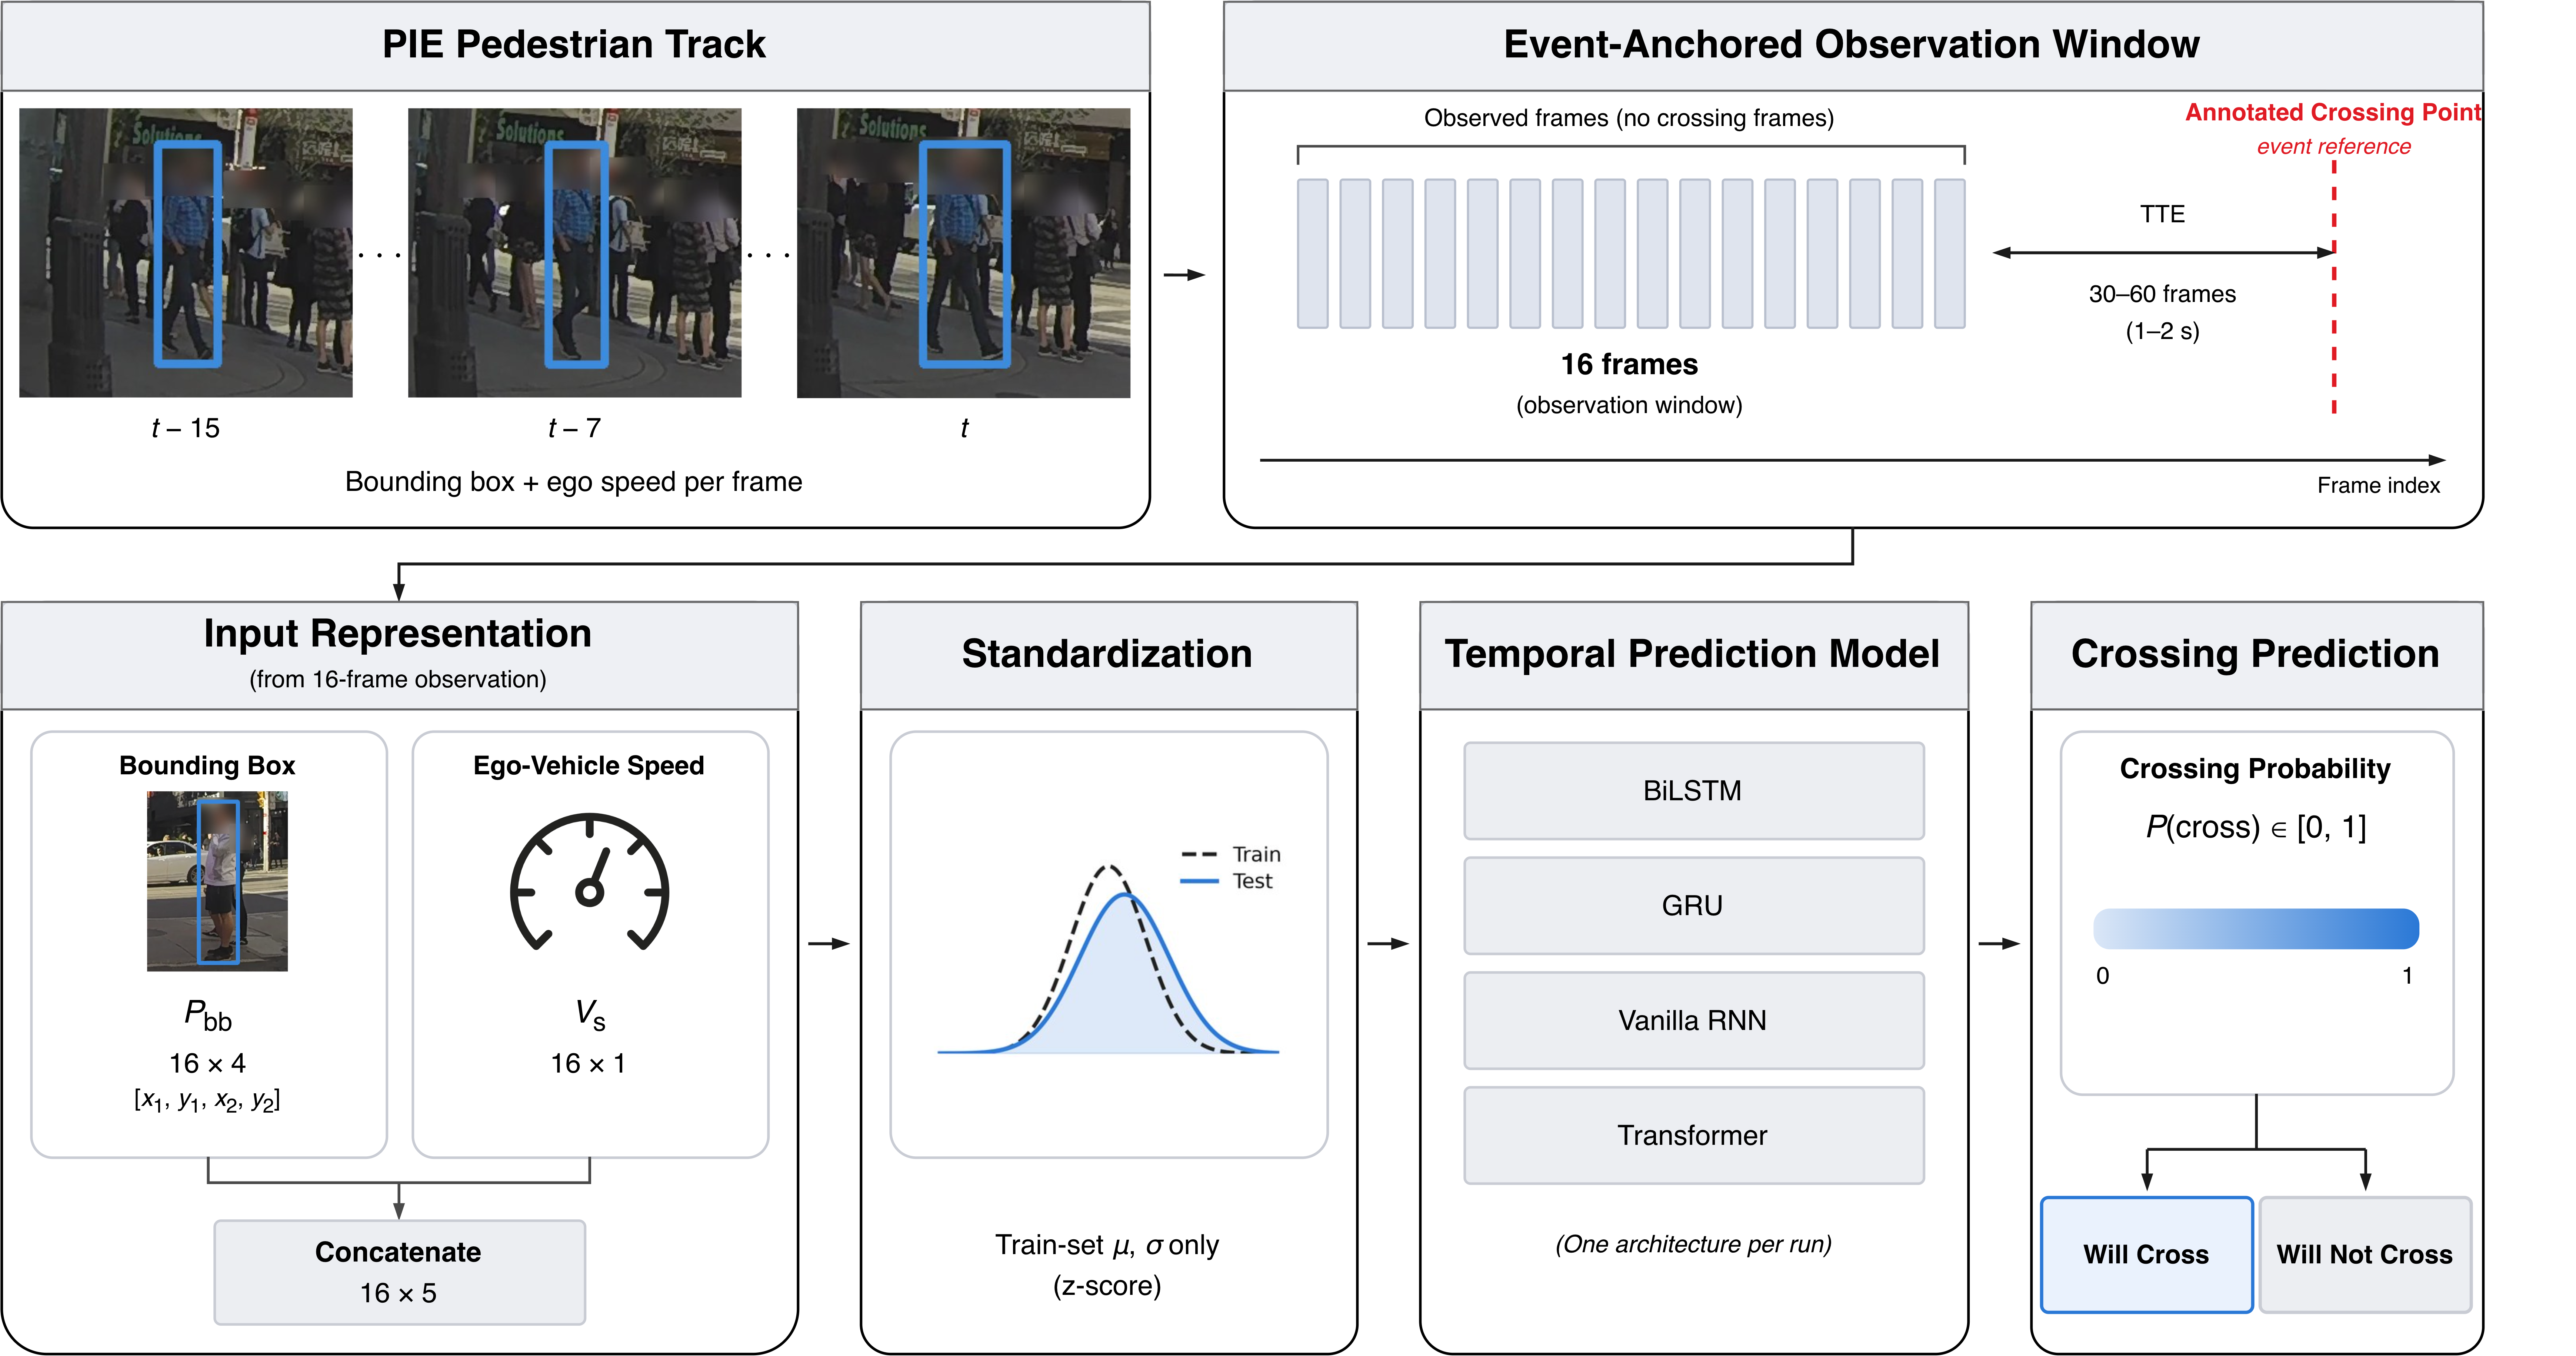
\includegraphics[width=\textwidth]{figures/fig2_method.png}
\caption{The pipeline from an annotated PIE track to a crossing decision. The sixteen observed frames end 30--60 frames before the crossing point, so none is a crossing frame. Box and ego speed form a $16 \times 5$ input, standardised on the training split.
\label{fig:method}}
\end{figure}

\subsection{Datasets and Data Partitioning}
The Pedestrian Intention Estimation (PIE) dataset~\citep{rasouli2019pie} was used as the
primary dataset. PIE provides pedestrian tracks with frame-level bounding boxes, behavioural
annotations, annotated crossing points, and synchronised ego-vehicle speed. Pedestrians with
a \texttt{crossing} label of $-1$ were excluded because they do not have a binary crossing
outcome. The remaining tracks were labelled as crossing or non-crossing according to PIE's
per-pedestrian \texttt{crossing} attribute. The prediction target in this study is therefore the observed crossing outcome rather than PIE's separately provided \texttt{intention\_prob} variable. A positive label indicates that the pedestrian is observed to cross in front of the ego vehicle, whereas a negative label indicates that the pedestrian does not cross. Because this label is defined at the pedestrian
track level, all observation windows extracted from the same pedestrian carry the same target label. The PIE recording sets were divided before observation-window generation. Sets 01, 02,
and 04 were used for training, sets 05 and 06 for validation, and set 03 for testing. Partitioning by recording set keeps all observations from a pedestrian within a single
partition and avoids sharing pedestrian tracks between training, validation, and test data.
The same partition was maintained throughout the PIE experiments.

JAAD~\citep{rasouli2017jaad} and IDD-PeD~\citep{bokkasam2025iddped} were used to examine the temporal procedure beyond PIE. JAAD supplies no ego-vehicle speed channel, only a small
set of coarse vehicle-action states, so the five-dimensional input used here cannot be
formed on it; JAAD was therefore used for an independent audit of generated observation windows only. IDD-PeD was used for both temporal auditing and cross-dataset evaluation
because it provides frame-level pedestrian behaviour together with per-frame vehicle-motion information. Dataset-specific partitions were kept at the recording-set level rather than
created by randomly dividing individual observation windows. Figure~\ref{fig:scenes} shows one annotated frame from each dataset.

\begin{figure}[H]
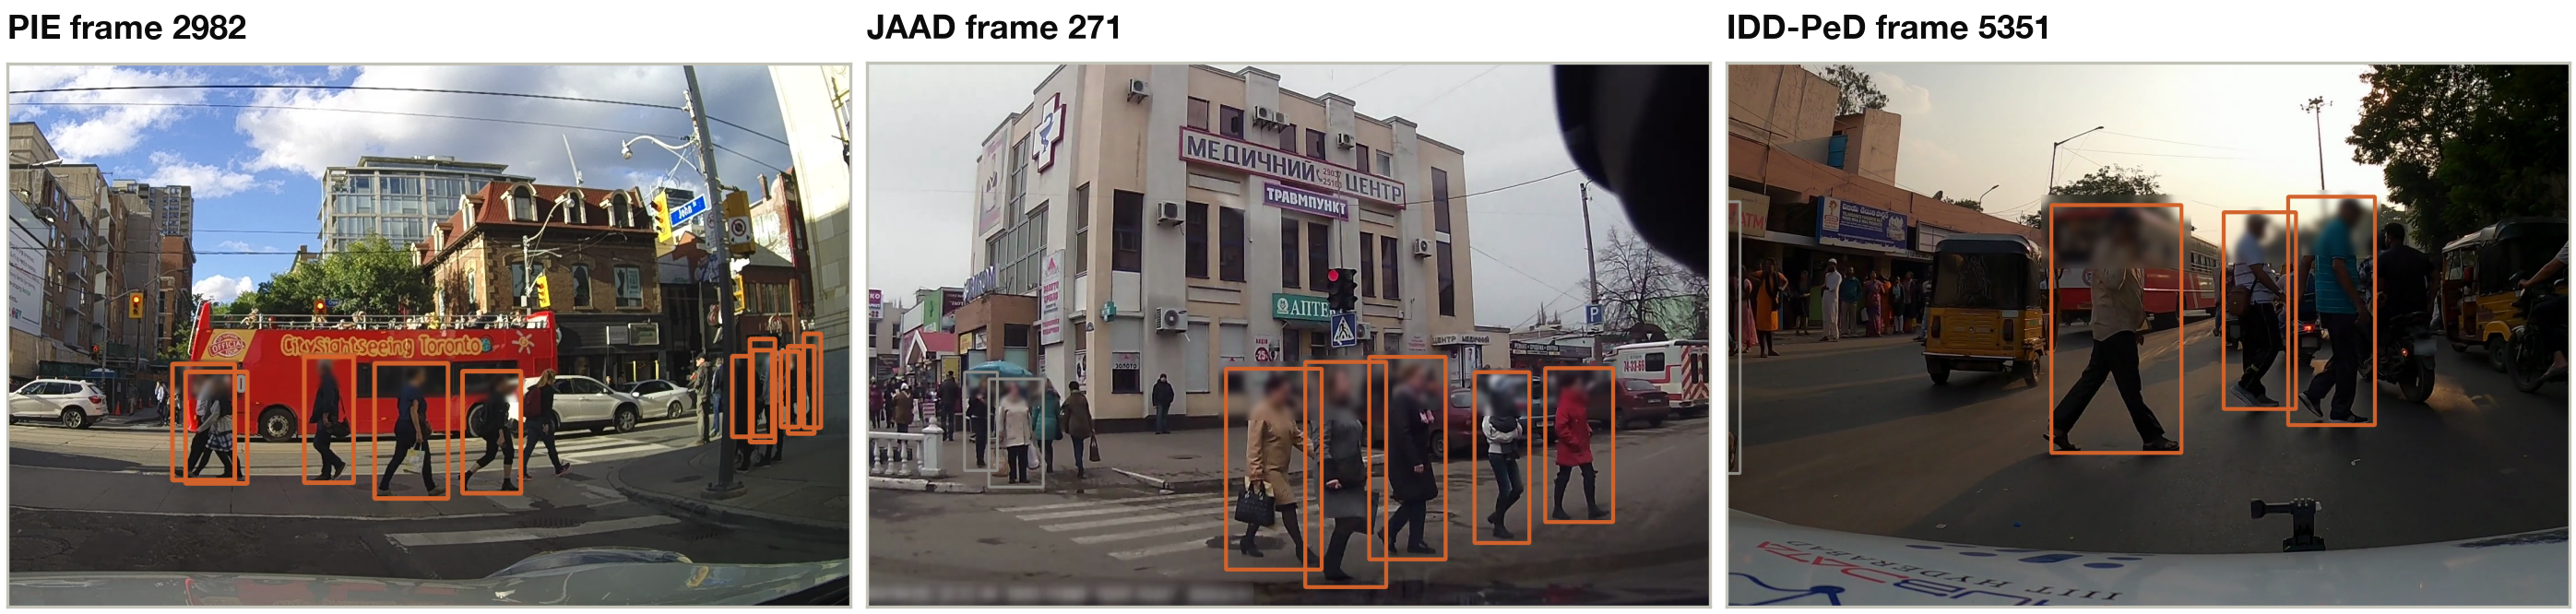
\includegraphics[width=\textwidth]{figures/fig7_scenes.png}
\caption{One annotated frame from each dataset. Boxes mark behaviour-annotated pedestrians,
coloured by the dataset's own eventual outcome rather than by any model prediction: orange
for pedestrians who cross, grey for those who do not. Faces were blurred.\label{fig:scenes}}
\end{figure}



\subsection{Temporal Data Extraction}

The prediction samples were constructed so that the temporal position of every observation could be checked relative to the pedestrian crossing event. Two extraction procedures were considered on PIE. The first reproduced the historical track-end procedure retained in the repository for temporal auditing. In this procedure, the temporal reference is derived from the end of the annotated pedestrian track and does not use the actual crossing point. The second procedure uses PIE's annotated \texttt{crossing\_point} as the event reference and
forms the main event-anchored dataset. For event-anchored extraction, the frames of each pedestrian track were first ordered and divided into contiguous segments. The segment containing the annotated \texttt{crossing\_point} was retained, and frames after this point were removed. Fixed-length observation windows were then sampled from the admissible interval before the event. A pedestrian was excluded when the available contiguous pre-event sequence was too short to form a complete observation window within the required prediction horizon. This procedure was applied independently within the fixed training, validation, and test partitions. Temporal validity was verified from the generated windows rather than assumed from the sampling rule. Each observed frame was compared with the corresponding frame-level crossing annotation. A window was classified as temporally contaminated when at least one of its input frames was already annotated as crossing. This audit was performed separately for the historical and event-anchored extractions. The same frame-level principle was used when auditing JAAD and IDD-PeD.

%For IDD-PeD, the supplied crossing reference was additionally checked against the first frame at which a crossing behaviour was annotated. Two event definitions were examined: the provided \texttt{crossing\_point} and a stricter reference defined by the earlier of the provided crossing point and the first annotated crossing frame. This allowed temporal validity to be assessed using the dataset's observed crossing state rather than relying on the event marker alone. Event anchoring fixes the position of a positive window relative to the crossing action, but not the position of the two classes relative to each other. This class-dependent sampling phase was examined using the distance from the end of the observation to the end of the full pedestrian track. The variable was used only as a diagnostic of the sampling procedure and was not supplied to the prediction models. A phase-matched control was then constructed to reduce this difference. Positive windows were retained at their original event-relative positions. The target-distance distribution was estimated from the positive training windows only. Negative windows in the training, validation, and test partitions were then resampled earlier in their tracks using this fixed training-derived distribution. Each target was restricted to the temporal range available in the corresponding negative track, and only complete consecutive observation windows were retained. Negative tracks that could not provide a valid window within this common temporal support were excluded. The phase-matched data preserved the original recording-set assignments and the positive event definition. The neural models were trained again on the resulting phase-matched data rather than applying models trained under the event-anchored sampling procedure. This design changes the negative sampling phase while keeping the modeling and evaluation procedure unchanged. Figure~\ref{fig:anchors} illustrates the three anchoring rules and the resulting position of the observation window for each class.
{\color{blue}
For IDD-PeD, the supplied crossing point was checked against the first frame annotated as crossing. Two event references were examined: the supplied crossing point and the earlier of this point and the first annotated crossing frame. This allowed temporal validity to be assessed from the frame-level crossing annotations rather than the event marker alone.

On PIE, event anchoring placed observation windows before the crossing event. However, crossing and non-crossing pedestrians could still be observed at different stages of their tracks. This difference was examined using the number of frames from the last observed frame to the end of the full pedestrian track. This temporal distance was used only to assess the sampling procedure and was not supplied to the prediction models. To reduce the difference between the classes, a phase-matched control was constructed. Windows from crossing pedestrians were kept at their original positions relative to the event. The distribution of this distance was estimated from the training windows of crossing pedestrians only. Windows from non-crossing pedestrians in the training, validation, and test partitions were then resampled earlier in their tracks using this fixed distribution. Each sampled distance was restricted to the temporal range available in the corresponding non-crossing track, and only complete windows of consecutive frames were retained. Non-crossing tracks that could not provide such a window were excluded. The original recording-set assignments and crossing-event definition were preserved. The neural models were retrained on the phase-matched data, while the modelling and evaluation procedures remained unchanged. Figure~\ref{fig:anchors} contrasts the historical track-end extraction with event anchoring combined with phase matching.
Figure~\ref{fig:phase} shows the timing distributions under event anchoring and phase matching.
\par
}

\begin{figure}[H]
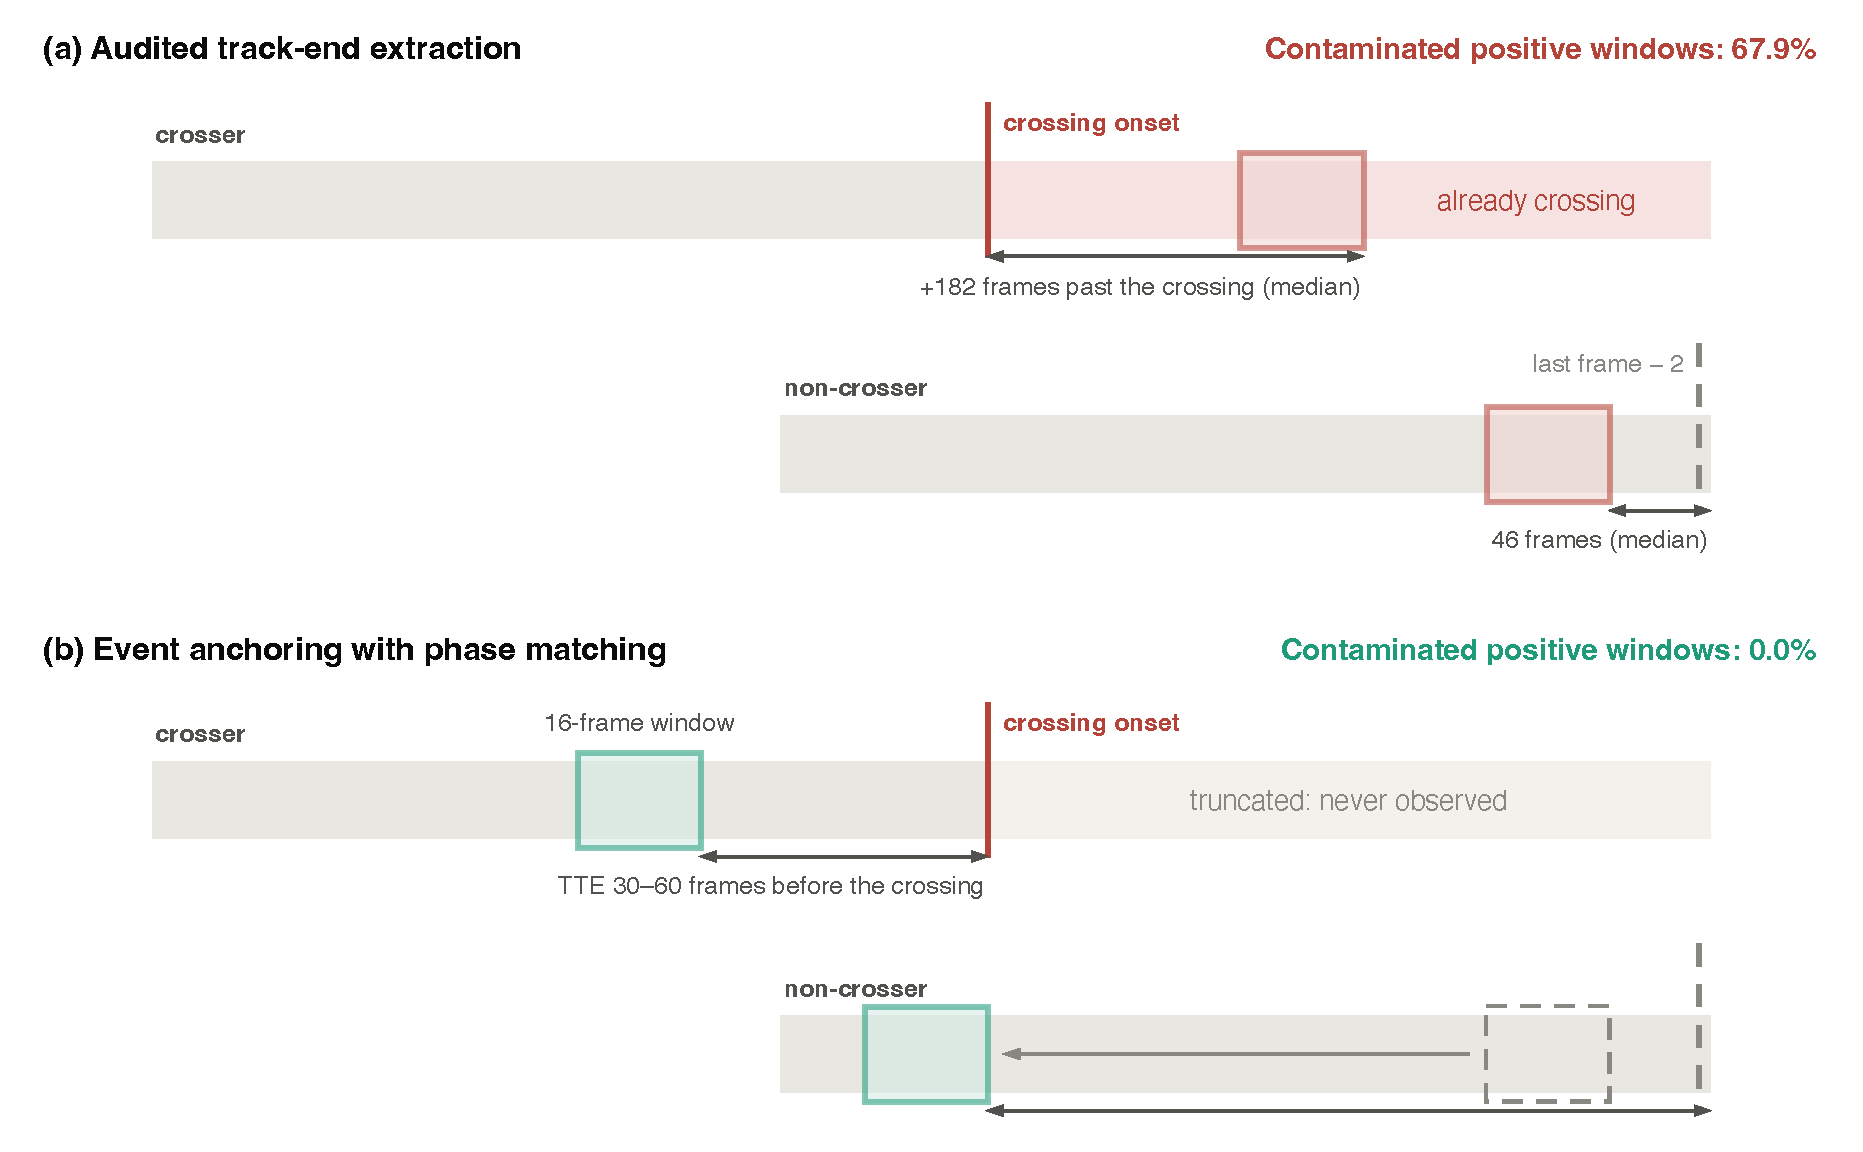
\includegraphics[width=\textwidth]{figures/fig3_anchors.pdf}
\caption{PIE observation-window sampling:
(\textbf{a}) audited track-end extraction;
(\textbf{b}) event anchoring with phase-matched
non-crossing windows.\label{fig:anchors}}
\end{figure}

\subsection{Input Representation and Preprocessing}

Each frame of an observation window was represented by the pedestrian bounding box and
the synchronised ego-vehicle speed. The frame-level input vector was

\begin{equation}
    \mathbf{x}_{t}
    =
    \left[
    x_{1,t},
    y_{1,t},
    x_{2,t},
    y_{2,t},
    v_{\mathrm{ego},t}
    \right],
\end{equation}

where $(x_{1,t},y_{1,t})$ and $(x_{2,t},y_{2,t})$ denote the upper-left and lower-right
coordinates of the pedestrian bounding box, respectively, and $v_{\mathrm{ego},t}$ denotes the ego-vehicle speed at frame $t$. Bounding-box coordinates were retained in the original image coordinate system, and vehicle speed was aligned with the pedestrian observations by frame identifier.

For the neural sequence models, each input channel was standardised using statistics estimated only from the training partition, and those statistics were then applied unchanged to the validation and test partitions. The contribution of ego-vehicle speed was examined by repeating each neural model with only the four bounding-box coordinates. The full-input condition used the same bounding-box coordinates together with ego-vehicle speed. This five-dimensional versus four-dimensional ablation was performed on both the event-anchored PIE data and the phase-matched PIE control. Within each protocol, the two input conditions used the same recording-set
partitions, family-specific configuration, five random seeds, training procedure, checkpoint-selection rule, and evaluation procedure. Removing the speed channel changed only the input projection, reducing the model by 64 parameters. The same box-only and box-plus-speed comparison was also evaluated for the in-domain IDD-PeD experiments using the corresponding IDD-PeD partitions.


\subsection{Temporal Prediction Models}

Four neural sequence-model families were evaluated: a bidirectional long short-term memory network (BiLSTM), a bidirectional gated recurrent unit (GRU), a bidirectional un-gated recurrent neural network (RNN), and a Transformer. All models received the same type of frame sequence and produced a single probability for the binary crossing outcome. For the recurrent models, the frame-level features were first projected to a learned representation and then processed in both temporal directions. The resulting sequence representation was passed to a binary classification layer. The BiLSTM and GRU use gated recurrent units, whereas the vanilla RNN provides an un-gated recurrent reference. The Transformer replaces recurrent processing with positional encoding and self-attention over the observation sequence.



\subsection{Training and Evaluation}
\label{sec:methods-training-evaluation}

%Model parameters were learned from the training partition, while the validation partition was used for model configuration, checkpoint selection, and the classification operating point. 
\textcolor{blue}{Model parameters were learned from the training partition, while the validation partition was used to configure the models, select checkpoints, and determine the classification operating point.} The test partition was reserved for final evaluation and was not used to fit model parameters, preprocessing statistics, or decision thresholds. Class imbalance was handled using a positive-class weight calculated from the training partition, recomputed whenever the sampling procedure changed the training-set class distribution. Each selected configuration was trained from several random initialisations. Model performance was evaluated using ROC-AUC, PR-AUC, F1-score, and accuracy, the first two from prediction probabilities and the last two at operating thresholds selected from validation predictions.

Observation windows from the same pedestrian overlap in time and carry one track-level target, so they were treated as a cluster rather than as independent observations. %Confidence intervals and %model contrasts were computed by resampling pedestrians, with all %windows of a selected pedestrian resampled %together~\citep{fieldwelsh2007}. 
\textcolor{blue}{Mean metrics were calculated across the five seed runs, and
standard deviations summarised seed-to-seed variability.
For statistical comparisons, test probabilities were averaged
across the five seeds for each model and input condition.
Reported contrasts therefore compare ensemble metrics, which
can differ from differences between the per-seed means in the
tables. Their 95\% confidence intervals were estimated by
resampling pedestrians, with all windows of a selected pedestrian
resampled together~\citep{fieldwelsh2007}.
The trained models and validation-selected thresholds remained
fixed during resampling, so these intervals describe test-sample
uncertainty for the fixed ensembles.} Models evaluated on the same test pedestrians used shared resamples so that the comparison remained paired, whereas the two sampling protocols were resampled independently because their eligible pedestrians differ. Multiple contrasts were adjusted using the Holm--Bonferroni procedure within a predefined family of comparisons for each analysis, with accuracy recorded descriptively and excluded from every family. One further set of experiments was exploratory and is reported in Section~\ref{sec:limitations} rather than among the results: the PIE-trained models, their preprocessing statistics, and their operating point were transferred to IDD-PeD unchanged, with pedestrian boxes mapped to the PIE image coordinate frame, and separate in-domain models were trained on the IDD-PeD partitions only.



\section{Experimental Settings}
\label{sec:experimental-settings}

All the experiments were run on a CPU using the computing environment listed in Table~\ref{tab:hardware}. The main PIE dataset contained 4,906 observation windows, with 2,178 used for training, 634 for validation, and 2,094 for testing. Each observation contained 16 consecutive frames. Windows were sampled with a stride of eight frames, and the final observed frame was positioned 30--60 frames before the crossing reference, corresponding to approximately 1--2~s at 30 frames per second.

\begin{table}[htbp]
\centering
\caption{Computing environment used for all the experiments.}
\label{tab:hardware}
\begin{tabular}{ll}
\toprule
\textbf{Component} & \textbf{Specification} \\
\midrule
Reference machine & Apple M4 MacBook Air, CPU execution \\
Python & 3.13.5 \\
PyTorch & 2.12.0 \\
NumPy & 2.4.6 \\
pandas & 3.0.3 \\
SciPy & 1.17.1 \\
scikit-learn & 1.9.0 \\
Matplotlib & 3.11.0 \\
\bottomrule
\end{tabular}
\end{table}

% All four model families used the same data partitions, preprocessing rules, training procedure, validation procedure, and test-evaluation procedure. The configurations of each family were selected using the validation data. Model capacity was not constrained to be identical across families; each family was evaluated using its selected configuration. All models were trained with binary cross-entropy loss and the Adam optimizer. The batch size was 32, training was limited to 100 epochs, and the weight decay was $10^{-5}$. Early stopping was applied after 15 epochs without improvement in validation AUC. The learning rate was reduced by a factor of 0.5 after five epochs without improvement. The positive-class weight was calculated from the training split and was 1.682 for the main PIE data.

% The selected BiLSTM, GRU, and vanilla RNN configurations each used two bidirectional recurrent layers with a hidden size of 256 and dropout of 0.2. The BiLSTM and vanilla RNN used a learning rate of $10^{-4}$, while the GRU used $10^{-3}$. Their five-dimensional frame input was first projected to 64 dimensions using a linear layer followed by a ReLU activation. The selected Transformer used a model dimension of 128, four attention heads, four encoder layers, a feed-forward dimension of 512, and dropout of 0.1. Sinusoidal positional encoding and last-token pooling were used, with a learning rate of $10^{-3}$.

% Each recurrent family had 36 searched configurations. The Transformer search contained 78 configurations, including 36 architecture configurations and 42 additional recipe or transfer configurations. The final Transformer was included in the 36 architecture configurations. The final comparison therefore used the validation-selected configuration of each family rather than forcing identical hyperparameters or model capacity across families.
% Each configuration was trained using five random seeds, ${42,0,1,2,3}$. For each run, the checkpoint with the highest validation AUC was retained. The validation probabilities from the five runs of each model family were averaged, and one classification threshold was selected by maximising F1 on these pooled validation predictions. The selected threshold was then fixed for test evaluation. For the ego-speed ablations, the box-plus-speed and box-only models each used a threshold selected from their own pooled validation predictions.

% The phase-matched control contained 4,520 windows, with 2,084 used for training, 563 for validation, and 1,873 for testing. %Its positive-class weight was recomputed from the corresponding training split which was 1.5665. 
% \textcolor{blue}{Its positive-class weight was recalculated from the phase-matched training split and was 1.5665.} The phase-matched test split contained 476 pedestrians, with a positive prevalence of 36.4\%. Statistical comparisons used 10,000 pedestrian-cluster bootstrap samples. Models evaluated on the same test pedestrians used the same bootstrap samples, while the original and phase-matched protocols were resampled independently because their eligible test populations differed. Holm--Bonferroni correction was applied at $\alpha=0.05$ within the predefined comparison families described in Section~\ref{sec:methods-training-evaluation}.

All four model families used the same data partitions, preprocessing rules, and training, validation, and test-evaluation procedures. Configurations were selected using validation data without requiring equal model capacity across families. All models were trained with binary cross-entropy loss and the Adam optimizer, using a batch size of 32, a maximum of 100 epochs, and a weight decay of $10^{-5}$. Training stopped after 15 epochs without improvement in validation AUC. The learning rate was reduced by a factor of 0.5 after five epochs without improvement. The positive-class weight was calculated from the training split and was 1.682 for the event-anchored data. The selected BiLSTM, GRU, and vanilla RNN models used two bidirectional recurrent layers with a hidden size of 256 and dropout of 0.2. Their five-dimensional frame inputs were projected to 64 dimensions through a linear layer followed by ReLU. The BiLSTM and vanilla RNN used a learning rate of $10^{-4}$, while the GRU used $10^{-3}$. The Transformer used a model dimension of 128, four attention heads, four encoder layers, a feed-forward dimension of 512, and dropout of 0.1. It used sinusoidal positional encoding, last-token pooling, and a learning rate of $10^{-3}$. The search evaluated 36 configurations for each recurrent family and 78 for the Transformer. The Transformer search included 36 architecture configurations and 42 additional configurations for training or transfer; the selected configuration came from the architecture search. Each configuration was trained using five random seeds, ${42,0,1,2,3}$. The checkpoint with the highest validation AUC was retained for each run. For each model family, validation probabilities were averaged across the five runs, and a classification threshold was selected by maximising F1. This threshold was fixed for test evaluation. In the ego-speed ablations, the box-plus-speed and box-only models each used a threshold selected from their own averaged validation predictions. The phase-matched control contained 4,520 windows: 2,084 for training, 563 for validation, and 1,873 for testing. Its positive-class weight was recalculated from the training split and was 1.5665. The phase-matched test split contained 476 pedestrians, with a positive prevalence of 36.4\%. Statistical comparisons used 10,000 pedestrian-clustered bootstrap samples. Models evaluated on the same test pedestrians shared bootstrap samples, while the event-anchored and phase-matched protocols were resampled independently because their eligible test populations differed. Holm--Bonferroni correction was applied at $\alpha=0.05$ within the comparison families defined in Section~\ref{sec:methods-training-evaluation}.

\subsection{Qualitative Evaluation with Detected Tracks}

A separate qualitative evaluation was conducted to examine the trained prediction system using automatically detected and tracked pedestrians rather than annotated pedestrian boxes. Pedestrians were detected with a YOLO detector and associated across frames using ByteTrack. The resulting tracked boxes were combined with the recorded ego-vehicle speed and provided to the frozen five-seed ensemble using the same 16-frame input format, training-split normalization statistics, and classification threshold used in the quantitative evaluation. This evaluation was not used to calculate test metrics or to compare model performance. It was used only to observe the behaviour of the trained prediction system when pedestrian tracks were obtained from detection and tracking rather than from annotations.


\section{Results}\label{sec:results}

The temporal audit first examined whether the observation windows contained frames from the crossing action. Under the historical PIE track-end extraction, 387 of 570 positive sequences (67.9\%) contained at least one frame in which the pedestrian was already annotated as crossing. In 369 of those 570 sequences (64.7\%), all 16 observed frames were already inside the crossing period, and only 8.4\% of the 570 retained at least 30 frames of genuine look-ahead before crossing onset. The temporal reference occurred a median of 182 frames after crossing onset, and the last observed pedestrian geometry showed strong class separation, with rank-biserial effect sizes of $+0.654$ for box area, $+0.629$ for box height, and $+0.485$ for the lower box edge. The event-anchored extraction removed this direct overlap. The annotated \texttt{crossing\_point} coincided with the first frame labelled as crossing for 516 of 519 crossing pedestrians (99.42\%) and was never earlier than the frame-level onset, and none of the 4,906 generated observation windows contained a frame labelled as crossing. The corresponding effect sizes decreased to $+0.247$ for box area, $+0.211$ for box height, and $+0.090$ for the lower box edge, and the horizontal box-centre effect decreased from $-0.186$ to $-0.018$. Anchoring on the annotated event therefore removed both the crossing frames and most of the static geometric separation between the two classes.

The frame-level audit showed that the same general problem can occur outside PIE, although the appropriate event reference differed between datasets. Under naive extraction, 93.0\% of the 460 positive JAAD windows and 81.3\% of the positive IDD-PeD windows contained at least one crossing frame. Event-based JAAD extraction produced 972 windows with no observed contamination. On IDD-PeD, directly using the released \texttt{crossing\_point} reduced contamination but still left 29.6\% of positive windows affected, and only the earlier of the supplied crossing point and the first frame-level crossing onset produced a clean set, of 7,318 windows. Table~\ref{tab:temporal-audit} summarises the audit for every dataset and anchoring rule.

\begin{table}[htbp]
\centering
\caption{Frame-level temporal-validity audit across the evaluated datasets. Contamination
indicates that at least one frame in the observation window was already annotated as
crossing.}
\label{tab:temporal-audit}
\begin{tabular}{llcc}
\toprule
\textbf{Dataset} & \textbf{Temporal anchor} &
\textbf{Generated samples} & \textbf{Contamination} \\
\midrule
PIE & Historical track-end & 570 positive sequences & 67.9\% of positives \\
PIE & \texttt{crossing\_point} & 4,906 windows & 0.0\% \\
JAAD & Naive anchor & 460 positive windows & 93.0\% of positives \\
JAAD & Event anchor & 972 windows & 0.0\% \\
IDD-PeD & Track-end & 8,651 windows & 81.3\% of positives \\
IDD-PeD & \texttt{crossing\_point} & 7,919 windows & 29.6\% of positives \\
IDD-PeD & Earlier event/onset & 7,318 windows & 0.0\% \\
\bottomrule
\end{tabular}
\end{table}

The four neural families were next compared on the event-anchored PIE test set using the common training and evaluation procedure, with their five-seed results shown in Table~\ref{tab:model-results}. The vanilla RNN produced the highest mean ROC-AUC ($0.9481\pm0.0058$), F1-score ($0.8487\pm0.0154$) and accuracy ($0.8996\pm0.0117$), while the Transformer produced the highest mean PR-AUC (0.8964); the GRU reached an F1-score of $0.8419\pm0.0083$ and the BiLSTM reached $0.8276\pm0.0174$. The pedestrian-clustered analysis showed that 7 of the 18 neural family--metric contrasts remained statistically significant after Holm correction on the event-anchored data. The vanilla RNN had higher AUC than the BiLSTM ($\Delta=0.0225$, 95\% CI $[0.0114,0.0340]$, $p_{\mathrm{Holm}}=0.0036$) and the GRU ($\Delta=0.0121$, 95\% CI $[0.0042,0.0217]$, $p_{\mathrm{Holm}}=0.0120$). Its F1-score was also higher than the BiLSTM ($\Delta=0.0320$, 95\% CI $[0.0164,0.0490]$, $p_{\mathrm{Holm}}=0.0036$) and the GRU ($\Delta=0.0185$, 95\% CI $[0.0062,0.0323]$, $p_{\mathrm{Holm}}=0.0224$), and its PR-AUC was higher than the GRU ($\Delta=0.0125$, 95\% CI $[0.0037,0.0231]$, $p_{\mathrm{Holm}}=0.0480$). The Transformer had higher AUC than the BiLSTM ($\Delta=0.0231$, 95\% CI $[0.0128,0.0345]$, $p_{\mathrm{Holm}}=0.0036$) and than the GRU ($\Delta=0.0127$, 95\% CI $[0.0039,0.0235]$, $p_{\mathrm{Holm}}=0.0338$). These seven contrasts are the complete set that survived correction, and no statistically supported difference was detected between the Transformer and vanilla RNN for AUC, PR-AUC, or F1.

\begin{table}[htbp]
\centering
\caption{The four neural model families on the event-anchored PIE test set, each using
bounding boxes with ego-vehicle speed. Values are five-seed means $\pm$ standard deviations.
Accuracy is descriptive and was not included in any tested family.}
\label{tab:model-results}
\setlength{\tabcolsep}{5pt}
\begin{tabular}{lcccc}
\toprule
\textbf{Model} & \textbf{AUC} & \textbf{PR-AUC} & \textbf{F1} & \textbf{Accuracy} \\
\midrule
BiLSTM &
$0.9242\pm0.0086$ & $0.8688\pm0.0089$ & $0.8276\pm0.0174$ & $0.8826\pm0.0144$ \\
Transformer &
$0.9447\pm0.0090$ & $\mathbf{0.8964\pm0.0188}$ & $0.8250\pm0.0274$ & $0.8849\pm0.0230$ \\
GRU &
$0.9375\pm0.0029$ & $0.8890\pm0.0050$ & $0.8419\pm0.0083$ & $0.8945\pm0.0073$ \\
Vanilla RNN &
$\mathbf{0.9481\pm0.0058}$ & $0.8925\pm0.0062$ & $\mathbf{0.8487\pm0.0154}$ &
$\mathbf{0.8996\pm0.0117}$ \\
\bottomrule
\end{tabular}
\end{table}

%The event-anchored input ablation showed a positive contribution from ego-vehicle speed in both threshold-free metrics for all four neural families, but the magnitude depended strongly on the architecture. The five-dimensional minus four-dimensional mean PR-AUC differences were $+0.2189$, $+0.1527$, $+0.1217$, and $+0.0565$ for the BiLSTM, vanilla RNN, GRU, and Transformer, respectively, and the corresponding mean AUC differences were $+0.1477$, $+0.0715$, $+0.0538$, and $+0.0156$. Ten of these 12 input contrasts remained significant after Holm correction on the pedestrian-clustered bootstrap. The speed channel raised PR-AUC for the BiLSTM ($\Delta=0.2100$, 95\% CI $[0.1490,0.2700]$, $p_{\mathrm{Holm}}=0.0024$), the vanilla RNN ($\Delta=0.1287$, 95\% CI $[0.0657,0.1987]$, $p_{\mathrm{Holm}}=0.0024$), and the GRU ($\Delta=0.0653$, 95\% CI $[0.0278,0.1112]$, $p_{\mathrm{Holm}}=0.0024$). The two contrasts that did not survive correction were both the Transformer's threshold-free metrics (PR-AUC $\Delta=0.0373$, 95\% CI $[-0.0079,0.0879]$; AUC $\Delta=0.0126$, 95\% CI $[-0.0041,0.0282]$; $p_{\mathrm{Holm}}=0.2128$ for both), so the Transformer was already the least speed-dependent family before any temporal control was applied. The apparent contribution of the same speed channel therefore varied substantially across the four neural models.

\textcolor{blue}{Under event anchoring, adding ego-vehicle speed increased the five-seed mean ROC-AUC and PR-AUC for all four models, although the gains varied by architecture. The mean PR-AUC increases were $+0.2189$, $+0.1527$, $+0.1217$, and $+0.0565$ for the BiLSTM, vanilla RNN, GRU, and Transformer, respectively; the corresponding ROC-AUC increases were $+0.1477$, $+0.0715$, $+0.0538$, and $+0.0156$. Statistical comparisons used metrics calculated from prediction probabilities averaged across the five seeds. These ensemble metrics can differ from the five-seed means. Across ROC-AUC, PR-AUC, and F1-score, 10 of the 12 comparisons remained significant after Holm correction using pedestrian-clustered bootstrap resampling. The ensemble PR-AUC increases were significant for the BiLSTM ($\Delta=0.2100$, 95\% CI $[0.1490,0.2700]$, $p_{\mathrm{Holm}}=0.0024$), vanilla RNN ($\Delta=0.1287$, 95\% CI $[0.0657,0.1987]$, $p_{\mathrm{Holm}}=0.0024$), and GRU ($\Delta=0.0653$, 95\% CI $[0.0278,0.1112]$, $p_{\mathrm{Holm}}=0.0024$). Only the Transformer's PR-AUC ($\Delta=0.0373$, 95\% CI $[-0.0079,0.0879]$) and ROC-AUC ($\Delta=0.0126$, 95\% CI $[-0.0041,0.0282]$) comparisons were not significant after correction ($p_{\mathrm{Holm}}=0.2128$ for both). The Transformer also showed the smallest mean gains from speed in both threshold-free metrics.}

Although the event-anchored PIE observations contained no crossing frames, their temporal positions still differed strongly between classes. The distance from the last observed frame to the end of the pedestrian track ranged from 32 to 62 frames for non-crossing observations, with a median of 46 frames, compared with 88 to 6,606 frames for crossing observations, with a median of 287 frames. The two distributions did not overlap, and this temporal variable alone separated the classes with an AUC of 1.0000. The phase-matched control, whose target distribution came from 812 positive training windows, reduced this class-dependent timing difference; the resulting dataset contained 4,520 windows, including 1,648 positive and 2,872 negative observations, and Figure~\ref{fig:phase} shows the distributions before and after the control. Temporal-position AUC decreased from 1.0000 to 0.7919 over the full dataset and to 0.8241 on the test split, so the difference was reduced but not eliminated.

\begin{figure}[H]
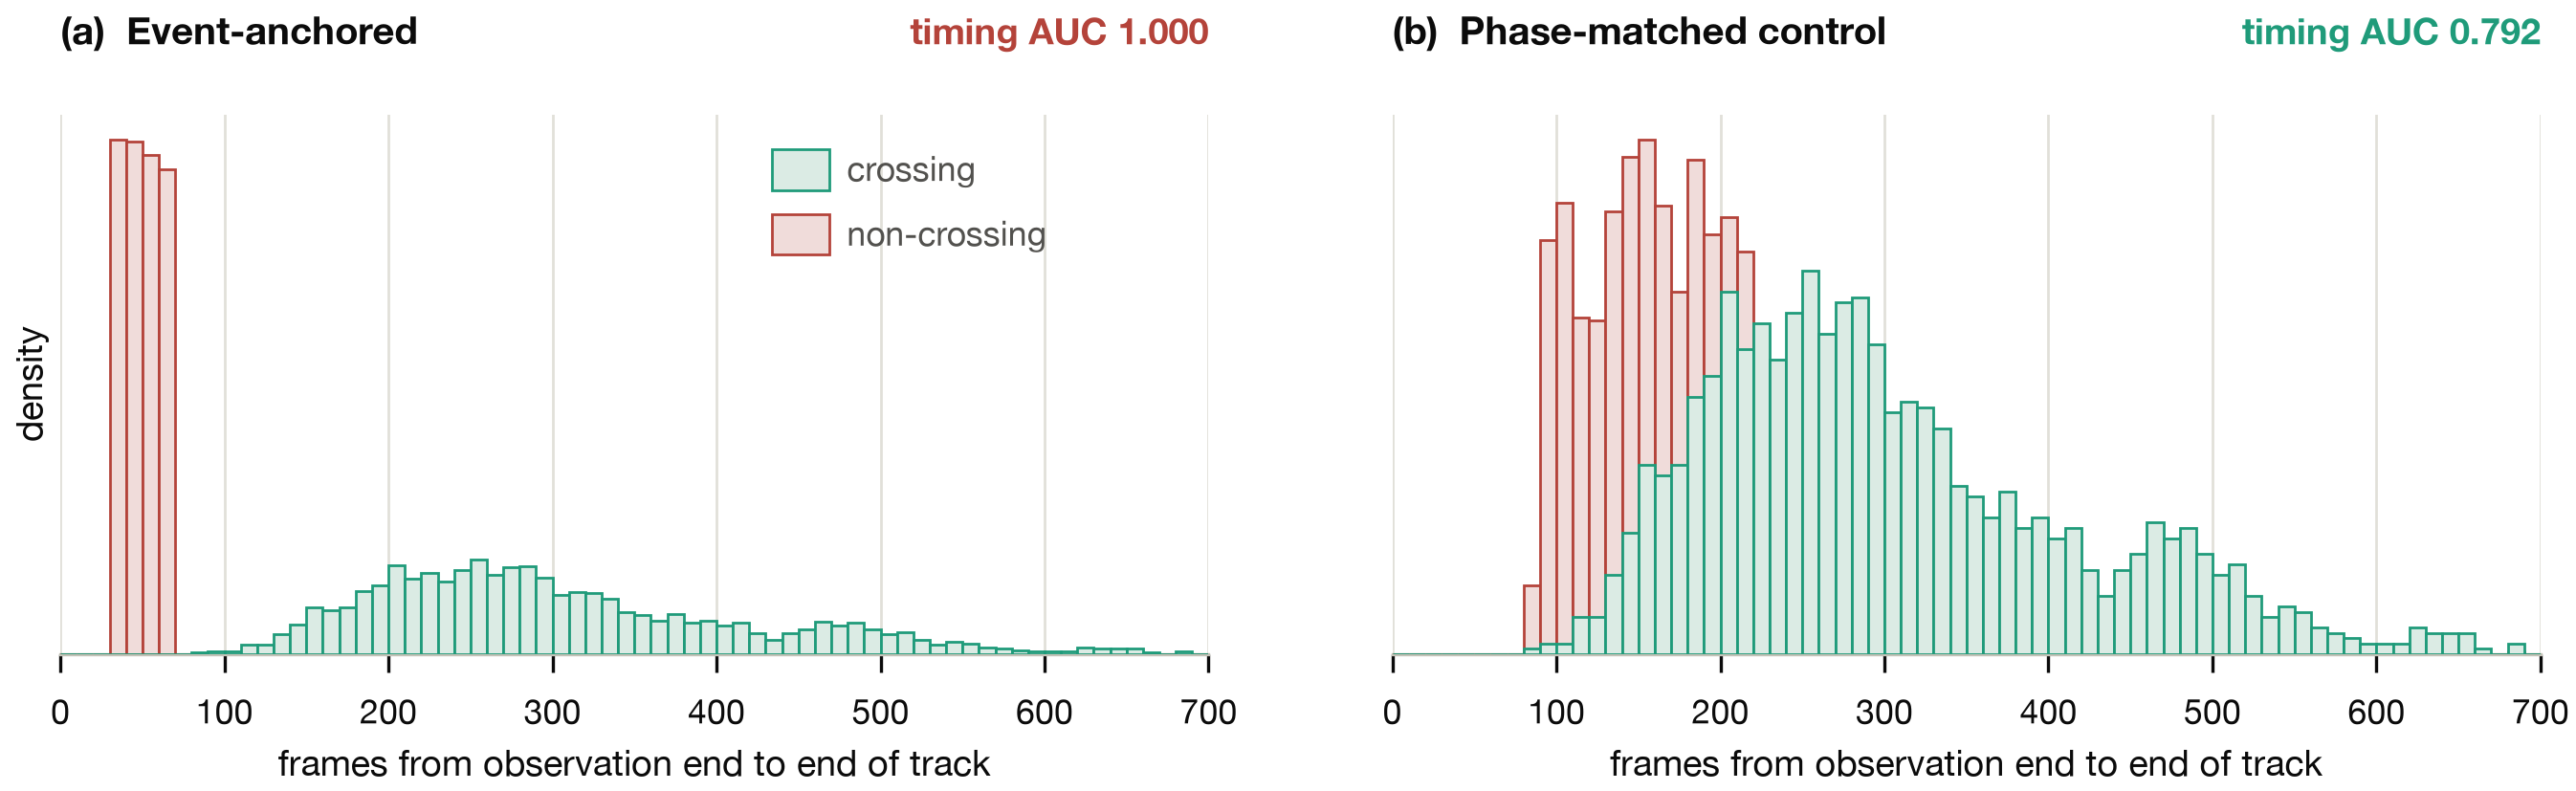
\includegraphics[width=\textwidth]{figures/fig4_phase_separation.png}
\caption{Distance from the end of the observation window to the end of the pedestrian track, by class. (\textbf{a}) Under event anchoring the two distributions do not overlap, so timing alone separates the classes. (\textbf{b}) After the negatives are re-drawn they overlap, reducing rather than removing the separation.\label{fig:phase}}
\end{figure}

Performance decreased after phase matching for all four full-input neural models on every metric. Table~\ref{tab:phase-control} shows the five-seed mean AUC, PR-AUC, F1-score, and accuracy under the two protocols; accuracy fell by 0.064 to 0.102, the largest drop being the Transformer's $0.8849 \rightarrow 0.7828$. The evidence for differences between neural families changed in the same way. Applying Holm correction to the same 18 family--metric comparisons gave 7 of 18 significant contrasts on the event-anchored data and 0 of 18 on the phase-matched data, the strongest phase-matched contrast being the Transformer--GRU AUC difference ($\Delta=0.0115$, uncorrected $p=0.0032$), which did not pass the first Holm threshold. Figure~\ref{fig:curves} shows the corresponding test-set operating characteristics under both protocols. Both the level of performance and the evidence for differences between families therefore moved with the sampling rule.

\begin{table}[htbp]
\centering
\caption{The four full-input model families before and after phase matching of the
negatives. Values are five-seed means; arrows read event-anchored to phase-matched. The
protocols are not paired, because their eligible pedestrian populations differ.}
\label{tab:phase-control}
\small
\setlength{\tabcolsep}{4pt}
\begin{tabular}{lcccc}
\toprule
\textbf{Model} & \textbf{AUC} & \textbf{PR-AUC} & \textbf{F1} & \textbf{Accuracy} \\
\midrule
BiLSTM &
$0.9242 \rightarrow 0.8923$ &
$0.8688 \rightarrow 0.7897$ &
$0.8276 \rightarrow 0.7698$ &
$0.8826 \rightarrow 0.8184$ \\
Transformer &
$0.9447 \rightarrow 0.8971$ &
$0.8964 \rightarrow 0.7947$ &
$0.8250 \rightarrow 0.7544$ &
$0.8849 \rightarrow 0.7828$ \\
GRU &
$0.9375 \rightarrow 0.8817$ &
$0.8890 \rightarrow 0.7684$ &
$0.8419 \rightarrow 0.7401$ &
$0.8945 \rightarrow 0.7964$ \\
Vanilla RNN &
$0.9481 \rightarrow 0.8872$ &
$0.8925 \rightarrow 0.7749$ &
$0.8487 \rightarrow 0.7553$ &
$0.8996 \rightarrow 0.8104$ \\
\bottomrule
\end{tabular}
\end{table}

\begin{figure}[htbp]
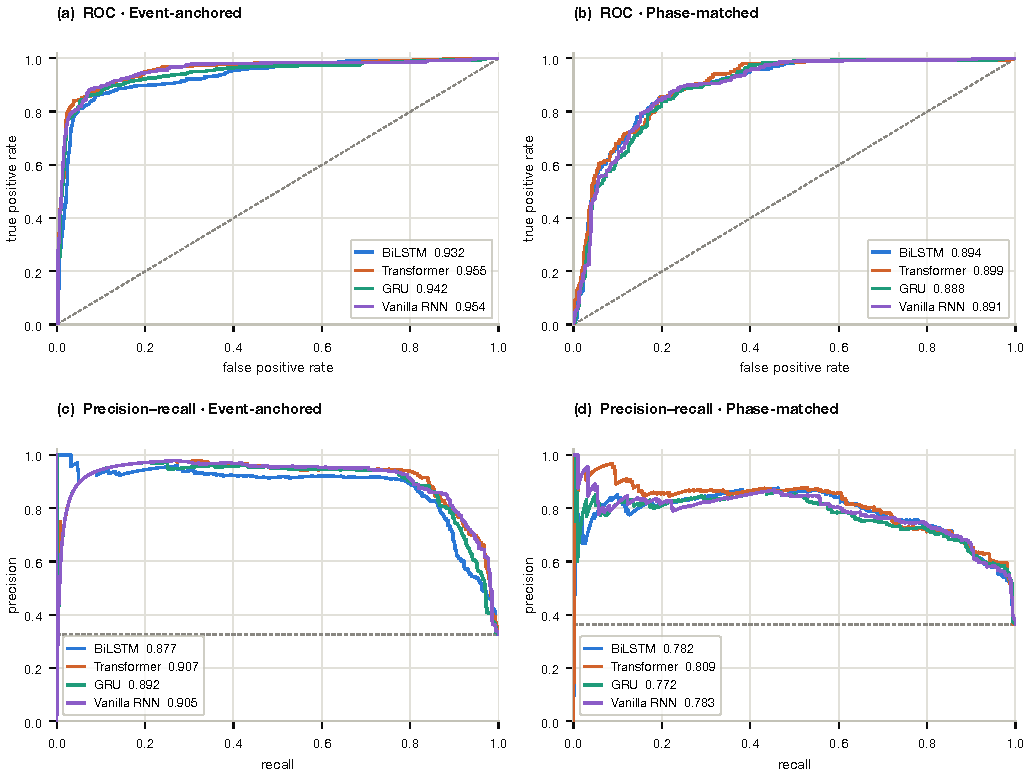
\includegraphics[width=\textwidth]{figures/fig5_curves.pdf}
\caption{Test-set operating characteristics under both protocols.
(\textbf{a},\textbf{b}) Receiver operating characteristic; (\textbf{c},\textbf{d})
precision--recall, dashed line at the positive prevalence. Curves use the five-seed
probability ensemble, so their areas differ slightly from the per-seed means in
Tables~\ref{tab:model-results} and~\ref{tab:phase-control}.\label{fig:curves}}
\end{figure}

The phase-matched ego-speed ablation produced a different result from the event-anchored ablation. Table~\ref{tab:speed-phase} reports the five-seed mean PR-AUC and AUC of each input arm under both protocols, together with the five-dimensional minus four-dimensional differences. Under event anchoring, all four differences were positive for both threshold-free metrics and 10 of the 12 contrasts survived correction. After phase matching the differences were small, their directions were mixed, and the pedestrian-clustered analysis found that none of the 12 five-dimensional versus four-dimensional contrasts across PR-AUC, AUC, and F1 remained significant after Holm correction. The result is therefore an absence of a statistically supported ego-speed effect under the phase-matched protocol; it is not evidence that removing the speed channel improves prediction. \textcolor{blue}{Comparing the two protocols, mean PR-AUC and ROC-AUC decreased for all
four box-plus-speed models. Changes in box-only performance varied
across model families. The BiLSTM box-only model improved in both
metrics (PR-AUC $0.6499 \rightarrow 0.8103$; ROC-AUC
$0.7765 \rightarrow 0.8970$), and the vanilla RNN box-only model
improved in PR-AUC ($0.7398 \rightarrow 0.7938$).
After phase matching, the box-only mean exceeded the box-plus-speed
mean in three of the four model families for each metric.
These descriptive changes indicate that the measured contribution
of ego-vehicle speed is sensitive to the sampling protocol.} %The absolute values distinguish two explanations for that change. If phase matching had simply made the task harder, both input arms would have declined together. Instead every box-plus-speed arm declined on both threshold-free metrics, while the box-only arm rose for the BiLSTM (PR-AUC $0.6499 \rightarrow 0.8103$; AUC $0.7765 \rightarrow 0.8970$) and the vanilla RNN (PR-AUC $0.7398 \rightarrow 0.7938$), and after matching the box-only arm was numerically ahead in three of the four families on both metrics. The two arms converge and, for most families, cross, so the performance that the speed channel appeared to contribute under event anchoring was tied to the class-dependent sampling phase rather than to a property of the input that survives temporal control.

\begin{table}[htbp]
\centering
\caption{\textcolor{blue}{Ego-vehicle speed ablation under the two PIE protocols. Values are five-seed means; $\Delta$ is box-plus-speed minus box-only, calculated from unrounded values.}}
\label{tab:speed-phase}
\small
\setlength{\tabcolsep}{4pt}
\begin{tabular}{llrrrrrr}
\toprule
& & \multicolumn{3}{c}{\textbf{Event-anchored}} &
\multicolumn{3}{c}{\textbf{Phase-matched}} \\
\cmidrule(lr){3-5}\cmidrule(lr){6-8}
\textbf{Metric} & \textbf{Model} &
\textbf{Box only} & \textbf{Box\,+\,speed} & \textbf{$\Delta$} &
\textbf{Box only} & \textbf{Box\,+\,speed} & \textbf{$\Delta$} \\
\midrule
\multirow{4}{*}{PR-AUC}
 & BiLSTM      & $0.6499$ & $0.8688$ & $+0.2189$ & $0.8103$ & $0.7897$ & $-0.0206$ \\
 & Vanilla RNN & $0.7398$ & $0.8925$ & $+0.1527$ & $0.7938$ & $0.7749$ & $-0.0188$ \\
 & GRU         & $0.7673$ & $0.8890$ & $+0.1217$ & $0.7634$ & $0.7684$ & $+0.0049$ \\
 & Transformer & $0.8399$ & $0.8964$ & $+0.0565$ & $0.7953$ & $0.7947$ & $-0.0006$ \\
\midrule
\multirow{4}{*}{ROC-AUC}
 & BiLSTM      & $0.7765$ & $0.9242$ & $+0.1477$ & $0.8970$ & $0.8923$ & $-0.0046$ \\
 & Vanilla RNN & $0.8766$ & $0.9481$ & $+0.0715$ & $0.8936$ & $0.8872$ & $-0.0064$ \\
 & GRU         & $0.8836$ & $0.9375$ & $+0.0538$ & $0.8871$ & $0.8817$ & $-0.0054$ \\
 & Transformer & $0.9291$ & $0.9447$ & $+0.0156$ & $0.8959$ & $0.8971$ & $+0.0012$ \\
\bottomrule
\end{tabular}
\end{table}

The directions of the threshold-dependent metrics were mixed in the phase-matched input ablation. The BiLSTM and vanilla RNN box-only arms had slightly higher mean PR-AUC and AUC but lower F1 than their full-input counterparts. %Each input arm used its own validation-%selected threshold, and for these two families the box-only %threshold was far lower than the full-input one ($0.486$ against %$0.217$ for the BiLSTM and $0.509$ against $0.174$ for the vanilla %RNN), so these differences reflect different operating points rather %than contradictory threshold-free rankings. 
\textcolor{blue}{Each input condition used its own validation-selected threshold.
For the BiLSTM, the thresholds were $0.217$ for box-only and
$0.486$ for box-plus-speed. For the vanilla RNN, they were
$0.174$ for box-only and $0.509$ for box-plus-speed.
Because F1 depends on the classification threshold, its ranking
can differ from those of PR-AUC and ROC-AUC.} None of these metric directions was statistically supported after Holm correction.

Running the trained ensemble on detected rather than annotated pedestrians reproduced the same dependence in a different setting. Figure~\ref{fig:demo} shows the detection-to-prediction output on three PIE test scenes. With the vehicle stationary, three crossing pedestrians were assigned probabilities between 0.86 and 0.90; in a second stationary scene, 11 of the 12 tracked pedestrians were flagged, with probabilities between 0.37 and 0.84. While the vehicle was moving at 14~km/h, a single crossing pedestrian received 0.84 and the remaining eleven received between 0.01 and 0.19. Across the complete tracked output the ensemble's predicted probability correlated with ego-vehicle speed at $r=-0.892$: it flagged 96.2\% of tracked pedestrians when the vehicle was stationary and 1.00\% when it travelled above 20~km/h. The deployed system therefore separates pedestrians between frames far more strongly than within them, which is the behaviour the phase-matched ablation predicts and is consistent with the speed channel carrying much of the apparent signal under the original sampling.

\begin{figure}[htbp]
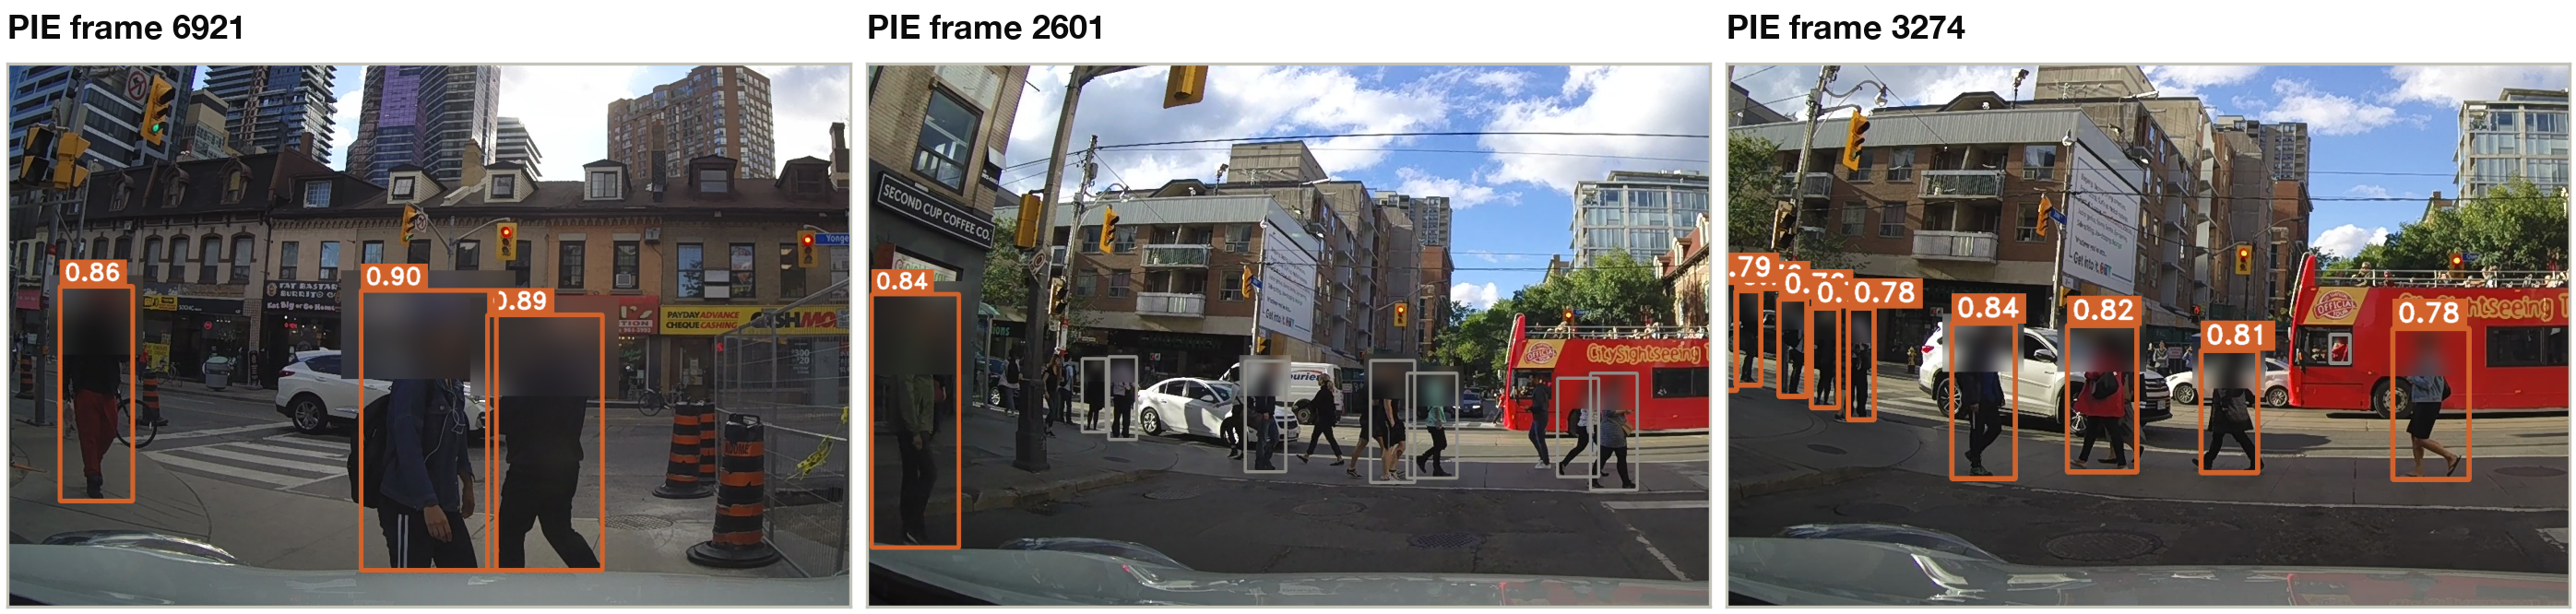
\includegraphics[width=\textwidth]{figures/fig6_demo.png}
\caption{Detection-to-prediction output on three PIE test scenes; boxes from the detector
and tracker, not annotation. Pedestrians predicted to cross are coloured with their
probability, the rest grey. The vehicle is stationary in scenes 1 and 3 and moving at
14~km/h in scene 2. Faces were blurred.\label{fig:demo}}
\end{figure}


\section{Discussion}
\label{sec:discussion}

%This research provides a frame-level method for testing the temporal validity of a pedestrian crossing-prediction benchmark, together with a sampling control that tests whether a reported result survives it. The temporal claims rest on five mechanisms: an audit of every observed frame against the dataset's own crossing annotation (Table~\ref{tab:temporal-audit}); recording-set partitions fixed before window generation, so no pedestrian appears in more than one partition; five random seeds for every configuration, reported as means and standard deviations (Tables~\ref{tab:model-results} and~\ref{tab:phase-control}); pedestrian-clustered bootstrap resampling with 10,000 replicates, which preserves the dependence between windows drawn from the same pedestrian; and Holm--Bonferroni correction within a predefined family of comparisons. Event-relative sampling is not itself new~\citep{kotseruba2021benchmark}; the contribution here is the direct measurement of whether the generated windows satisfy the pre-event requirement. That measurement remains necessary even when an event annotation is available: PIE's \texttt{crossing\_point} matches the frame-level onset closely and produces no contamination, whereas a literal use of the same field on IDD-PeD leaves crossing frames in 29.6\% of positive windows, and only the earlier of the supplied marker and the first frame annotated as crossing removes the overlap. The same temporal field therefore cannot be assumed to carry identical semantics across datasets. Removing those frames is also not sufficient. In the event-anchored PIE data the distance from the observation to track termination separates the classes perfectly, although this variable is never supplied to the models (Figure~\ref{fig:phase}), and reducing that separation lowers performance across all four full-input families on every metric (Table~\ref{tab:phase-control}).
\textcolor{blue}{This study combines a frame-level audit with a phase-matched control to examine how observation-window construction affects pedestrian crossing prediction. The findings are supported by fixed recording-set partitions, five random seeds, pedestrian-clustered bootstrap resampling with 10,000 replicates, and Holm--Bonferroni correction (Tables~\ref{tab:temporal-audit}, \ref{tab:model-results}, and~\ref{tab:phase-control}). Event-relative sampling is already established~\citep{kotseruba2021benchmark}; the contribution here is to verify whether the generated windows satisfy the pre-event requirement. On PIE, the annotated \texttt{crossing\_point} closely matches the first frame annotated as crossing and produces windows without crossing frames. On IDD-PeD, however, using the supplied \texttt{crossing\_point} leaves crossing frames in 29.6\% of positive windows. This contamination is removed by using the earlier of the supplied crossing point and the first annotated crossing frame. These results show that event markers must be checked against each dataset's frame-level annotations, even when the fields have the same name. Removing crossing frames does not ensure that crossing and non-crossing pedestrians are observed at comparable stages of their tracks. In the event-anchored PIE data, the distance from the last observed frame to the end of the track perfectly separates the classes, although this distance is not supplied to the models (Figure~\ref{fig:phase}). Phase matching reduces this timing difference, and performance is lower for all four models using bounding boxes and ego-vehicle speed on every reported metric (Table~\ref{tab:phase-control}).}


Both headline findings depend on that structure. Adding ego-vehicle speed raises both threshold-free metrics in every family under event anchoring, and 10 of the 12 input contrasts survive Holm correction; after phase matching none of the 12 survive (Table~\ref{tab:speed-phase}). %The absolute values indicate that this is not simply a %harder task: every box-plus-speed arm declines while the box-only %arm does not, so the two input conditions converge rather than %falling together.
\textcolor{blue}{From event anchoring to phase matching, mean PR-AUC and ROC-AUC
decreased for all four box-plus-speed models, whereas changes in
box-only performance varied across model families.
The differences between the two input conditions became smaller,
indicating that the measured contribution of ego-vehicle speed
is sensitive to the sampling protocol.} The architecture comparison moves the same way, from 7 of 18 family--metric contrasts surviving correction to none (Figure~\ref{fig:curves}); what changes is the statistical evidence available to rank these temporal architectures, not a demonstration that the four families perform equally. Previous PIE-based studies report ego speed as an informative signal~\citep{lorenzo2021intformer,azarmi2024featureimportance}, and strong results are also reported from bounding-box sequences alone or from boxes combined with speed~\citep{achaji2022attention,chen2024pedcmt}; the present result does not show that ego-vehicle speed is uninformative in general, only that its apparent contribution on PIE depends strongly on the sampling protocol. Comparable sensitivity of model rankings to training and model-selection conditions is documented more broadly in machine learning~\citep{melis2018sota,lucic2018gans}, and these experiments add benchmark construction as a further factor of the same kind. %The detector-to-prediction evaluation shows consistent pattern with this interpretation: When the trained ensemble was evaluated using detector- and tracker-generated pedestrian boxes rather than ground-truth annotations, it flagged almost every tracked pedestrian when the vehicle was stationary and almost none when the vehicle was moving. (Figure~\ref{fig:demo}), offering little discrimination between the pedestrians visible in a single frame. The results therefore place the emphasis on benchmark construction rather than on selecting a single best temporal model, and frame-level validation of observation windows should be treated as part of the evaluation procedure.
\textcolor{blue}{The detector-to-prediction demonstration used pedestrian bounding boxes obtained from a detector and tracker rather than from ground-truth annotations. Crossing predictions were more frequent when the vehicle was stationary than when its speed exceeded 20~km/h (Figure~\ref{fig:demo}). This pattern is consistent with an association between the predictions and ego-vehicle speed. The controlled benchmark results highlight the importance of observation-window construction when comparing temporal models. Frame-level validation of these windows should therefore form part of the evaluation procedure.}

\subsection{Limitations}
\label{sec:limitations}

%Even after correcting the observation windows and controlling the sampling phase, this study faces several limitations. The temporal audit covers PIE, JAAD, and IDD-PeD, which shows that crossing-frame contamination is not specific to one dataset. Beyond that audit, however, the analysis is confined to PIE, because neither external dataset supports the phase-matched comparison: JAAD provides no ego-vehicle speed channel, and the relation between IDD-PeD's released \texttt{crossing\_point} and the observed crossing onset does not fully match the description in the original publication~\citep{bokkasam2025iddped}. Transfer of the PIE-trained models to IDD-PeD under one predefined mapping gives weak performance and is reported only as a limit on external validity, without the statistical procedure applied to the PIE experiments; substantial cross-dataset degradation has also been reported previously~\citep{gesnouin2022assessing}. In addition, the phase-matched control reduces but does not eliminate the class-dependent temporal difference, partly because non-crossing tracks are shorter, and moving negative observations earlier can change pedestrian distance and bounding-box scale. %The resulting changes therefore indicate sensitivity to the sampling phase rather than an exact attribution to one isolated shortcut. 
%\textcolor{red}{These changes show that the measured performance is sensitive to the sampling phase.} Furthermore, the prediction target is the observed crossing outcome rather than latent pedestrian intention~\citep{rasouli2024diving}, and the input is restricted to pedestrian bounding boxes and ego-vehicle speed, so the findings should not be assumed to hold unchanged for systems using appearance, body pose, or scene semantics. Future work will repeat the phase-matched comparison on an external dataset that provides synchronised ego-vehicle motion, examine domain adaptation in place of zero-shot transfer, and extend the audit and the sampling control to richer input modalities.
\textcolor{blue}{Even after correcting the observation windows and controlling the sampling phase, this study has several limitations. The temporal audit covers PIE, JAAD, and IDD-PeD, but the controlled phase-matched comparison is limited to PIE. JAAD provides no ego-vehicle speed channel, and the relation between IDD-PeD's released \texttt{crossing\_point} and the observed crossing onset does not fully match the description in the original publication~\citep{bokkasam2025iddped}. Exploratory IDD-PeD experiments included transfer of PIE-trained models and separate in-domain training. Transfer under one predefined mapping gave weak performance and was reported only as a limit on external validity, without the statistical analysis applied to the PIE experiments. Substantial cross-dataset degradation has also been reported previously~\citep{gesnouin2022assessing}. In addition, the phase-matched control reduced but did not eliminate the timing difference between the classes, partly because non-crossing tracks were shorter. Moving non-crossing observations earlier could also change pedestrian distance and bounding-box scale. \textcolor{red}{These changes show that the measured performance is sensitive to the sampling phase.} Furthermore, the prediction target is the observed crossing outcome rather than latent pedestrian intention~\citep{rasouli2024diving}, and the input is restricted to pedestrian bounding boxes and ego-vehicle speed, so the findings should not be assumed to hold unchanged for systems using appearance, body pose, or scene semantics. Future work will repeat the phase-matched comparison on an external dataset that provides synchronised ego-vehicle motion, examine domain adaptation in place of zero-shot transfer, and extend the audit and the sampling control to richer input modalities.}


\section{Conclusions}\label{sec:conclusions}

%This study examines how the temporal construction of a pedestrian crossing-prediction benchmark affects what that benchmark measures. The task is multimodal: the model combines observed pedestrian geometry with synchronised ego-vehicle motion, and published systems justify each added stream by the gain it produces. A frame-level audit of the generated observation windows on PIE, JAAD, and IDD-PeD shows that a window anchored on the end of a pedestrian track already contains frames of the crossing action, and that the overlap is removed only when the window is anchored on the observed crossing onset. Event anchoring alone is not sufficient. Crossing and non-crossing pedestrians remain observed at systematically different phases of their tracks, and this timing is predictive without ever being supplied to the model. A phase-matched negative control that reduces this difference also removes the apparent advantage of the vehicle-motion stream over pedestrian geometry alone, together with the statistically supported differences among the BiLSTM, GRU, vanilla RNN, and Transformer encoders. The implication extends beyond this task: a per-modality ablation measures what a stream contributes only when the two classes are sampled from comparable points in the pedestrian--vehicle interaction. Overall, the findings indicate that temporal validity and class-dependent sampling phase should be verified from the frames supplied to the model and reported alongside modality ablations, so that a measured cross-modal gain reflects future crossing prediction rather than information introduced by sample construction.

\textcolor{red}{This study examined how the temporal construction of a pedestrian crossing-prediction benchmark affects the prediction task and the evaluation of different input modalities. The analysis of PIE, JAAD, and IDD-PeD showed that observation windows constructed from the end of a pedestrian track can already include frames in which the crossing action has started. Anchoring the window at the observed crossing onset removes this direct overlap, but it does not by itself make the comparison between crossing and non-crossing samples temporally balanced. The two classes can still be observed at different stages of their pedestrian tracks, and this difference can provide useful information to the model even though the observation phase is not explicitly included as an input. A phase-matched control was therefore used to reduce this class-dependent temporal difference. After phase matching, the apparent contribution of ego-vehicle speed was no longer statistically supported, and none of the tested differences among the four temporal model families remained statistically supported after Holm correction. These results show that the measured contribution of an input feature and the comparison between model families can depend on how the observation windows are constructed. These findings suggest that pedestrian crossing benchmarks should be checked at the frame level before evaluating different input modalities or model architectures. Overall, the results indicate that the timing and temporal composition of the observation window are important parts of the crossing-prediction task, and that reported gains from additional input information should be interpreted in relation to how the samples are constructed.}


\vspace{6pt}


\authorcontributions{Conceptualization, M.A.S., and N.T.; methodology, M.A.S., and N.T.; software, M.A.S.; validation, M.A.S.; formal analysis, M.A.S., and N.T.; investigation, M.A.S.; resources, M.A.S.; data curation, M.A.S.; writing---original draft preparation, M.A.S.; writing---review and editing, N.T., M.A.S.K, and K.Y.; visualization, M.A.S.; supervision, N.T., M.A.S.K, and K.Y.; project administration, M.A.S., and N.T. All authors have read and agreed to the published version of the manuscript.}

\funding{This research received no external funding.}

\institutionalreview{Not applicable. This study is a secondary analysis of publicly available datasets and involved no new experiments on humans or animals.}

\informedconsent{Not applicable.}

\dataavailability{The study used three publicly available datasets, obtained from their original authors: PIE (\url{https://data.nvision2.eecs.yorku.ca/PIE_dataset/}), JAAD (\url{https://data.nvision2.eecs.yorku.ca/JAAD_dataset/}), and IDD-PeD (\url{https://cvit.iiit.ac.in/research/projects/cvit-projects/iddped}).}



\conflictsofinterest{The authors declare no conflicts of interest.}

\abbreviations{Abbreviations}{%
The following abbreviations are used in this manuscript:\\
\noindent
\begin{tabular}{@{}ll}
AUC & Area under the curve\\
BiLSTM & Bidirectional long short-term memory\\
CI & Confidence interval\\
CPU & Central processing unit\\
GRU & Gated recurrent unit\\
IDD-PeD & India Driving Dataset --- Pedestrian\\
JAAD & Joint Attention in Autonomous Driving\\
LSTM & Long short-term memory\\
PIE & Pedestrian Intention Estimation dataset\\
PR-AUC & Area under the precision--recall curve\\
RNN & Recurrent neural network\\
ROC-AUC & Area under the receiver operating characteristic curve\\
TTE & Time to event\\
\end{tabular}
}

%=================================================================
\begin{adjustwidth}{-\extralength}{0cm}

\reftitle{References}

\bibliography{references}

\PublishersNote{}
\end{adjustwidth}
\end{document}
